% Tento soubor nahraďte vlastním souborem s obsahem práce.
%=========================================================================
% Autoři: Michal Bidlo, Bohuslav Křena, Jaroslav Dytrych, Petr Veigend a Adam Herout 2019
\chapter{Úvod}
Nacházíme se v době rychlého vývoje techniky, který pronikl i do našich domácností. Každým dnem roste počet zařízení denní potřeby, která jsou připojená do celosvětové sítě -- internetu. Spolu s tímto trendem roste také komfort a možnosti bydlení, které z toho plynou. Díky tak rychlému rozvoji automatizace je možné provádět úkoly, které by dříve ani nebyly možné. Internet věcí lidem umožňuje vykonávat úkony -- jako vypínat spotřebiče při opuštění domácnosti, nastavit efektivní režim vytápění před příjezdem domů, či například zajistit zabezpečení celé domácnosti. 

Na trhu se nachází nejrůznější typy systémů domácí automatizace. V závislosti na ceně je možné pořídit jednoduchá zařízení, jako jednotlivé zásuvky či světla, až po různá komplexní řešení určená k zabudování do rozvaděčů domácnosti za účelem ovládání celé domácnosti. Komplexní řešení mohou pokrývat řadu různých snímačů a zařízení, které spolu mohou vytvořit opravdu automatizovaný dům. Přestože jde vývoj rychle dopředu, tak u komplexnějších systémů je cena velmi vysoká a většina domácností se tak bude muset bez chytrých zařízení obejít. 

A právě kvůli zajímavosti těchto systémů a jejich doposud vysoké ceně jsem se i já rozhodl v této práci zabývat možnostmi ovládání zařízení na dálku, potažmo možností jejich automatizace. V rámci práce bych chtěl vyvinout takový komplexní systém, který by byl použitelný v praxi a zároveň příliš nezatížil kapsu uživatele. Systém bude postaven na platformách Raspberry Pi a ESP8266, protože jsou cenově dostupné a mají velkou podporu ze strany uživatelů. Ke komunikaci mezi sebou budou tyto platformy využívat Wi-Fi, jelikož již samy o sobě mají potřebné prostředky a protokol CoAP, který je k podobným aplikacím určený. Systém bude sice využívat Raspberry Pi (jelikož se jedná o levné a energeticky relativně nenáročné zařízení), ale budu jej realizovat tak, aby byl multiplatformní (alespoň tam, kde to bude mít smysl). Grafické rozhraní pro komunikaci s uživatelem bude mít responzivní design. Kromě toho bude bude systém fungovat jak v rámci sítě internet (bude jej tedy možné ovládat na dálku, například z práce), tak i v lokální síti. Nebude tedy bezprostředně závislý na internetovém připojení. Veškerý kód, který v rámci práce vytvořím, bych chtěl uvolnit jako open source a nadále jej vyvíjet.


\chapter{Automatizace domácnosti}
Následující část je shrnutím současného stavu v oblasti chytré či automatizované domácnosti. Není encyklopedickým výkladem problematiky, ale souhrnem informací, které mají k práci bezprostřední vztah. Nejprve je zde vysvětlení základních pojmů, jako internet věcí, chytrá domácnost apod. Následuje pojednání o tom, jaké jsou dnes možnosti využití automatizace domácnosti, jaké přináší výhody a co patří mezi obvyklé funkce či mechanismy, které se v chytrých domácnostech využívají. Druhá podkapitola je věnována některým existujícím řešením chytrých domácností, které je možné si pořídit.

\section{Internet věcí a automatizace domácnosti}
\subsection*{Internet věcí a chytrá zařízení}
K automatizaci domácnosti neodmyslitelně patří tzv. Internet of Things (IoT), tedy internet věcí, který celý koncept automatizace významně rozšiřuje. Zatímco pod pojmem automatizace je možné si představit jakoukoli automatizovanou činnost, internet věcí označuje systém propojení různých zařízení, aplikací, snímačů a akčních členů, které mezi sebou mohou navzájem komunikovat a reagovat na sebe. Mezi aplikace konceptu internetu věcí patří široké spektrum odvětví jako chytrý průmysl, chytrá města, chytré zemědělství, chytré zdravotnictví, nebo konečně chytré domácnosti \cite{IoT}.

\subsection*{Automatizace domácnosti a chytrý dům}
Automatizace domácnosti spočívá v automatizování činností, které řídí domácnost, normálně vykonávané člověkem. Můžeme ji definovat jako mechanismus, který nahrazuje lidskou námahu (z ovládání domácnosti), natolik, nakolik je to jen možné \cite{HomeAutomationRPI}. V souvislosti s tím někdy hovoříme o inteligentní, řízené či chytré domácnosti. Jedná se o kolekci zařízení a (pod)systémů, které jsou schopny spolu komunikovat či fungovat nezávisle. Automatizovaný „dům budoucnosti“ slibují výrobci domácích zařízení prakticky již téměř od počátku minulého století \cite{HomeAutomationAndWiring}. Chytrá domácnost (či smart home) je také definována jako dům, vybavený výpočetní a informační technologií, které předvídá uživatelovy potřeby a odpovídá na ně, a přitom dbá na jeho pohodlí, bezpečnost a zábavu \cite{InsideTheSmartHome}. Často se tedy tyto dva pojmy (automatizovaná a chytrá domácnost) zaměňují. Chytrý dům však označuje spíše skupinu zařízení, schopných spolu nějakým způsobem (zejména po síti) komunikovat, zatímco automatizovaný dům je pojem, který popisuje, jakým způsobem jsou tato zařízení využívána \cite{SmartHomeVsHomeAutomation}.

\subsection*{Možnosti využití automatizace v domácnosti}
Automatizace v mnohém usnadňuje život a umožňuje provádění akcí, které by jinak byly prakticky nemožné (například zabezpečení domu, efektivní řízení vytápění domácnosti a spotřeby energie). V současné době patří automatizace domácnosti mezi rychle se rozvíjející technologie \cite{SmartHomeMarketForecast}.


Mezi typické aplikace automatizace domácnosti patří například:
\begin{itemize}
\item Zabezpečovací systém
\item Systém pro inteligentní vytápění a ventilaci (HVAC)
\item Zábava a multimédia
\item Komunikace
\item Osvětlení \cite{ClassificationOfFunctionsInSmartHome}
\item Ovládání spotřebičů
\item Samo-zavlažovací systémy \cite{HomeAutomationRPI}
\end{itemize}
A samozřejmě mnoho dalšího. Zmíněné aplikace jsou nejtypičtější, ke kterým se automatizace používá, ovšem na trhu vzniká čím dál více inovací, jako chytrá lednice či kávovar. 
\begin{figure}[hbt]
	\centering
	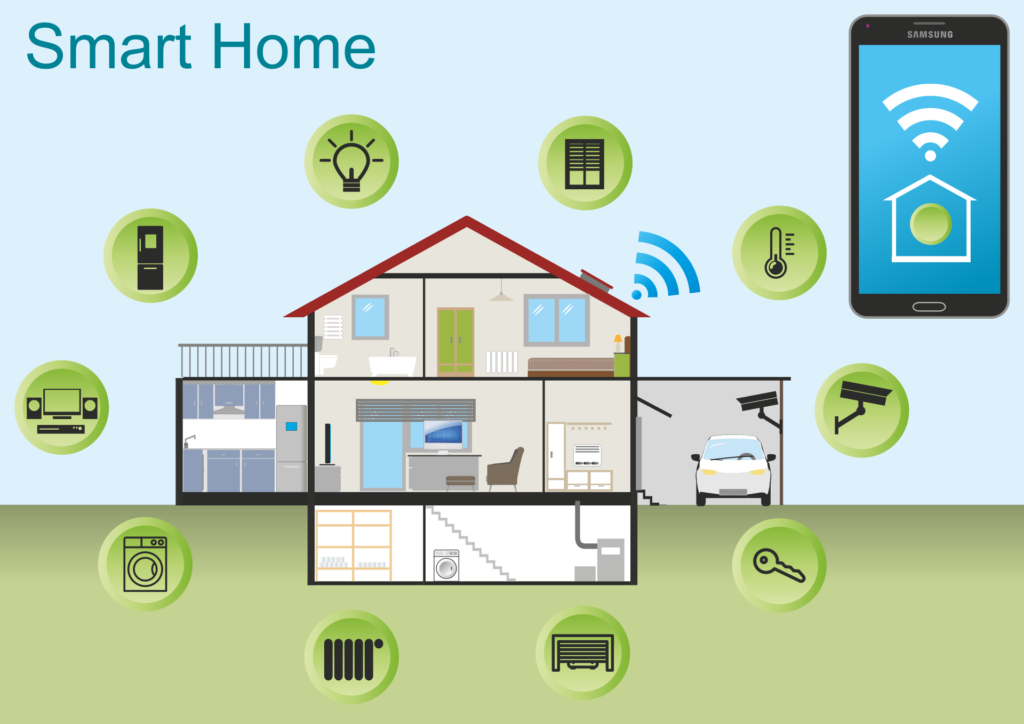
\includegraphics[scale=0.3]{obrazky/smart-home.png}
	\caption{Znázornění některých aplikací automatizované (či chytré) domácnosti. Převzato z \url{https://alejandraslife.com/smart-home-how-to-manage-your-energy/}}
	\label{homeAutomationExample}
\end{figure}
Na obrázku \ref{homeAutomationExample} můžeme vidět příklad chytrých prvků v domácnosti, z nichž mnohé je dnes již možné automatizovat.

\subsection*{Přínosy automatizace domácnosti}
Přidání inteligence do domácnosti přináší do života lidí řadu přínosů. Jde zejména o:

\begin{itemize}
\item Bezpečí – Chytré domy mohou používat různé senzory, které detekují nebezpečí a v souvislostí s nimi provést patřičné akce k jejich zabránění, případně minimalizaci škod. Příkladem mohou být záplavové a kouřové senzory, a v neposlední řadě také zabezpečovací systém domácnosti.
\item Komfort – Chytré domácnosti svými funkcemi nabízejí různé způsoby, jak jejich uživatelům zpříjemnit různé rutinní akce. Mohou se postarat o automatické nastavování žaluzií dle intenzity venkovního světla, přes dotykový displej na dálku ztlumit světlo či hlasovým pokynem uvést celý byt do jiného světelného režimu. 
\item Přehled o provozu – Systémy pro automatizaci domácnosti zahrnují i displeje s přehledem o stavu jednotlivých zařízení a čidel. Také je v některých systémech možné tyto informace sledovat i z chytrých telefonů, tabletů či počítačů (a to i vzdáleně). V některých komplexnějších systémech, které například zahrnují komunikaci přes mobilní sítě, je možné získávat přehled o provozu dokonce pomocí SMS zprávy (hodí se třeba při absenci internetového připojení) \cite{CoJeSmartHome}.
\item Úspora – V chytrých domácnostech je možné použít inteligentní vytápění domu založené na údajích z teplotních čidel, denní doby, případně nastaveném režimu domácnosti. Společnost ELKO EP odhaduje, že díky bezdrátové regulaci topení je možné ušetřit až 30\% nákladů na energii \cite{TopteSRozumem}. Úsporu rovněž zajistí automatizovaná světla, o kterých je možné mít v automatizované domácnosti vždy přehled, na dálku je zapínat/vypínat dle potřeby a rovněž je napojit na senzory, které je budou ovládat například na základě přítomnosti osob v místnosti.
\end{itemize}
    

\subsection*{Základní klasifikace chytré domácnosti}
Chytrou domácnost můžeme rozdělit dle kabeláže na:

\begin{itemize}
    \item Drátovou
    \item Bezdrátovou 
    \item Kombinovanou
\end{itemize}

Pokud má být domácnost komplexně automatizovaná, je často vhodnější mít celý systém propojený pomocí kabelů, jelikož takový systém bude spolehlivější a v případě potřeby nabízí rychlejší přenos dat (například pokud mají být součástí systému multimédia). Bezdrátové systémy se hodí zejména tam, kde není žádané zasahovat do elektroinstalace, či pokud uživatel potřebuje pouze jednodušší systém (například s ovládáním několika málo zařízení). Připravená kabeláž pro automatizaci domácnosti rovněž přináší výhodu snadnějšího řešení napájení jednotlivých chytrých zařízení, které se tak může rozvádět po bytě spolu s datovými kabely. Přitom pro propojení jednotlivých chytrých zařízení mezi sebou je možné využít různé typy kabelů (např. ethernetový) \cite{CoJeSmartHome}. Systémy s kombinovanou kabeláží pak vycházejí z klasické kabelové instalace s možností použití některých bezdrátových prvků (např. snímačů).

Dále můžeme systémy chytré domácnosti rozdělit na:
\begin{itemize}
\item Komplexní, dodávané specializovanými firmami
\item Sestavené uživatelem dle jeho potřeb
\end{itemize}

Nevýhodou systémů od specializovaných firem je především obvykle mnohem vyšší cena. Systémy sestavené uživatelem mohou využívat nějakého open source projektu a cena je tak daná jen použitými komponentami, které mohou být nepoměrně levnější oproti těm od specializovaných firem. Samozřejmě má toto řešení řadu nevýhod, jelikož si uživatel musí celý systém navrhnout a sestavit sám, a je tedy sám zodpovědný za jeho funkčnost \cite{DIYHomeAutomationVsProfessionallyInstalled}. 

Také můžeme systémy rozdělit na ty, které je možné ovládat hlasem a které nikoliv \cite{SmartHomeWithoutVoiceAssistant}.

\subsection*{Funkce používané v chytrých domácnostech}
V chytré domácnosti se často používají některé (či všechny) z následujících funkcí:

\begin{itemize}
\item Přímé ovládání spotřebičů
\item Nastavení scény
\item Podmínky \cite{CoJeSmartHomeHub}
\end{itemize}
Přímé ovládání spotřebičů se může provádět dálkovým ovládáním, kde se často využívá rádiové komunikace na frekvenci 443 MHz. Příkladem takového zařízení mohou být bezdrátové zásuvky od společnosti Emos \footnote{https://www.czc.cz/emos-dalkove-ovladane-zasuvky-bila/261962/produkt}.
Jiný způsob přímého ovládání rovněž zahrnuje použití jiného chytrého zařízení (například chytrého telefonu), pokud ovládané zařízení umí komunikovat pomocí stejné technologie (Wi-Fi či Bluetooth). Ovládání pomocí telefonu či podobného chytrého zařízení je možné i v případě, že ovládané zařízení neumí komunikovat stejnou technologií, ale v domácnosti existuje centrální prvek (tzv. hub), který podporuje obě technologie a funguje zde jako prostředník mezi oběma zařízeními. 
Funkce nastavení scény obvykle jistým způsobem sdružuje několik příkazů přímého ovládání. Může se jednat o scénu odchodu z domu, která vypne všechna světla, odpojí spotřebiče od elektrické sítě a aktivuje zabezpečovací systém. Některé chytré domácnosti mohou rozpoznat i večerní zapnutí televize a nastavit komfortním způsobem osvětlení.
Dalším principem uplatňovaným v chytré domácnosti je vlastní automatizace pomocí předem definovaných podmínek. Ty způsobí, že při určité akci systém zareaguje předem nastaveným způsobem. Například může systém díky nastaveným podmínkám udržovat teplotu v domácnosti na určité úrovni, nebo třeba zapnout venkovní osvětlení při detekci osoby za tmy. 

Zde stojí za zmínku webová služba IFTTT\footnote{https://ifttt.com/} (If This Then That), která přidává nastavování podmínek nový rozměr. Umožňuje propojit i spolu nijak nesouvisející služby či zařízení, které spolu běžně nekomunikují \cite{IFTTT}.

\subsection*{Komponenty chytré domácnosti}
Na trhu dnes existuje nepřeberné množství různých systémů. Tyto systémy se mezi sebou liší složitostí, cenou, dosahem apod. Chytrá domácnost může obsahovat některé z následujících komponent:

\begin{itemize}
\item Vstupní prvky (různá čidla, tlačítka, dotykové displeje…)
\item Výstupní prvky (světla, spotřebiče a různá zařízení)
\item Virtuální (hlasový) asistent
\item Centrální jednotka
\item Aplikace pro řízení domácnosti z chytrých zařízení (telefonu, tabletu, počítače…)
\end{itemize}

Systém nemusí obsahovat všechny zmíněné komponenty. Záleží na komplexnosti a složitosti daného systému. Některé systémy mohou jako centrální jednotku využívat virtuálního (hlasového) asistenta, příkladem může být Google Assistant či Amazon Alexa.

\section{Existující řešení chytrých domácností}
Dnes je na trhu nepřeberné množství systémů, lišících se v ceně, komplexnosti, způsobem komunikace a dalšími parametry. Není možné na jednotlivé systémy pohlížet stejně, protože každý systém má své vlastnosti a některé systémy je jen stěží možné srovnávat jako alternativy (stěží budeme srovnávat jako alternativu hotové řešení řady chytrých zařízení Home connect a systém Apple HomeKit, který propojuje různá chytrá zařízení). Některé systémy mezi sebou dokáží dokonce komunikovat a spolupracovat, například Apple HomeKit, obecně hlasoví asistenti či dříve zmíněná služba IFTTT, pomocí které je možné propojit některé systémy.
Jednou z nejčastějších aplikací automatizace, kterou různé systémy nabízejí, je ovládání světel a zásuvek. Mezi další aplikace patří ovládání hlavic radiátorů, chytré termostaty, ovládání ventilátorů, stínící techniky, alarm a jiné. Níže uvádím seznam některých systémů:
\begin{itemize}
\item Loxone
\item Jablotron
\item Apple HomeKit
\item Homeconnect
\item Kangtai 
\item a mnoho dalších
\end{itemize}
Kromě komerčně prodávaných systémů je k dispozici rovněž open source řešení, mezi známější patří například:
\begin{itemize}
\item Home Assistant
\item ESPHome
\item a mnoho dalších
\end{itemize}

Jednotlivé systémy se mezi sebou různým způsobem liší a není možné na ně pohlížet stejným způsobem. Každý systém má svůj způsob přidávání  nových zařízení, podporu, rozšiřitelnost, architekturu apod. V jistém smyslu speciálním typem systémů chytré domácnosti patří systém, využívající hlasového asistenta. Takový systém obvykle bývá snadno rozšiřitelný. Hlasovým asistentům je věnován závěr této podkapitoly.

\subsection*{Loxone}
Loxone je společnost, zaměřující se na automatizaci budov v rozsahu od malých bytů, přes hotely, až po rozsáhlé budovy a výrobní haly. Zaměřují se na širokou škálu aplikací, v oblasti automatizace domácnosti jde zejména o následující:
\begin{itemize}
\item Bezpečnost (pohybové senzory, dveřní a okenní senzory)
\item Přístup do budovy (přístup kódem zadávaným na klávesnici, NFC přívěškem či iButtonem, kamera)
\item Řízení filtrace bazénu
\item Větrání (automatické řízení ventilace, například na základě přítomnosti osoby, vlhkosti, teplotě…)
\item Regulace teploty (Loxone je možné připojit k jakémukoli zdroji teploty i chlazení)
\item Úspora energie (ovládání budovy k úsporám energie, např. automatické stínění jako ochrana přetopení ze slunečního tepla)
\item Osvětlení (ovládání bodového světla, LED pásků či Loxone závěsných světel)
\item Multimédia (ovládání audia, TV…)
\item Stínění (ovládání stínící techniky pomáhá při vytápění a chlazení v domě)
\item A díky rozšířením také mnoho dalšího \cite{ReseniLoxone}
\end{itemize}
Systém loxone se skládá z několika různých prvků:

\begin{itemize}
\item Miniserver
\item Rozšíření
\item Příslušenství (Loxone Tree zařízení)
\item Loxone Tree a Loxone Link kabeláž
\item Aplikace Loxone App a Loxone Config
\end{itemize}

Loxone prvky ke své činnosti potřebují tzv. miniserver. Ten v systému funguje jako centrální řídící jednotka, která se stará o automatizaci domácnosti. Loxone nabízí celkem 2 různé typy miniserveru, každou aktuálně v jedné ze dvou generací:

\begin{itemize}
\item Miniserver
\item Miniserver Go
\end{itemize}

Miniserver 1. i 2. generace mají oba 8 digitálních a 4 analogové vstupy a 8 digitálních výstupů (relé spínající max 250VAC/30VDC). Miniserver 1. generace má ještě navíc 4 analogové výstupy \cite{MiniserverDokumentace2}. Obě generace miniserveru slouží pro kabelovou komunikaci a jsou určené k instalaci na DIN lištu. Také jsou obě generace vybaveny rozhraním Loxone Link (pro kabelové připojení až 30 tzv. rozšíření) a LAN port (Fast ethernet). Pouze první generace obsahuje KNX rozhraní, naopak pouze druhá generace a verze Go obsahují již integrované rozhraní Loxone Tree (k první generaci je pro komunikaci po Loxone Tree sběrnici dodat rozšiřující modul) \cite{MiniserverDokumentace3}.

Pokud si uživatel přeje využívat bezdrátové komunikace mezi prvky systému Loxone (zejména pro bezdrátové ovládání), pak Loxone nabízí 2. typ miniserveru – Miniserver Go. Ten komunikuje s bezdrátovými periferiemi (rozšířeními a příslušenstvím) rádiovou komunikací na frekvenci 868MHz pro SRD pásmo pro Evropu (na 4 kanálech), případně 915MHz pro ITU region 2 (10 kanálů), s maximálním výkonem 3.16 mW \cite{MiniserverDokumentace}. Obsahuje také LAN port (Fast Ethernet) a rozhraní Loxone Link. K této verzi miniserveru je možné bezdrátově připojit až 128 periferií \cite{LoxonePresentMiniserverGo}. Druhá generace tohoto miniserveru pak přináší zejména výrazně vyšší výkon a bezpečnost \cite{NovyMiniserverGo}.

\begin{figure}[hbt]
	\centering
	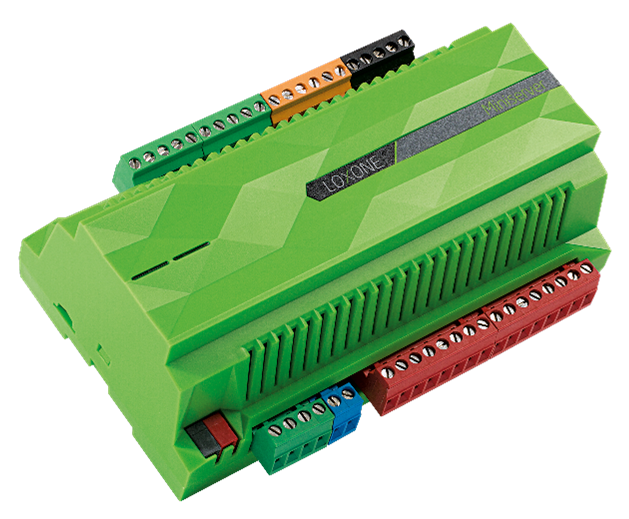
\includegraphics{obrazky/loxone-miniserver.png}
	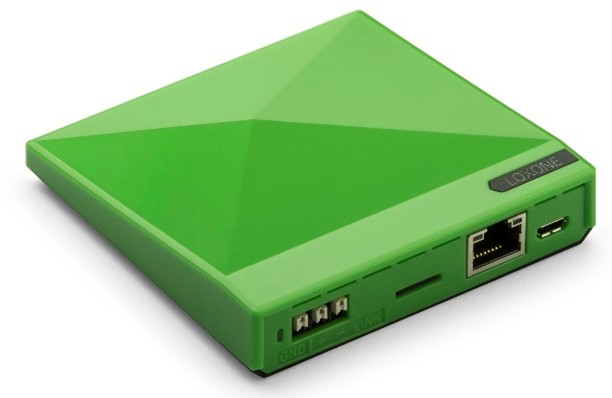
\includegraphics{obrazky/loxone-miniserver-go.jpg}
	\caption{Loxone Miniserver gen. 1 a Miniserver Go. Převzato z Loxone web}
	\label{miniserver}
\end{figure}


Všechny verze Miniserveru v sobě obsahují Loxone OS\footnote{OS - Operating system (operační systém)} s integrovaným webovým serverem, jsou konfigurovatelné z programu Loxone Config a ovladatelné přes mobilní aplikaci (Loxone App) \cite{MiniserverGo}. Všechny miniservery obsahují slot pro SD kartu (s firmwarem). 

\begin{figure}[hbt]
	\centering
	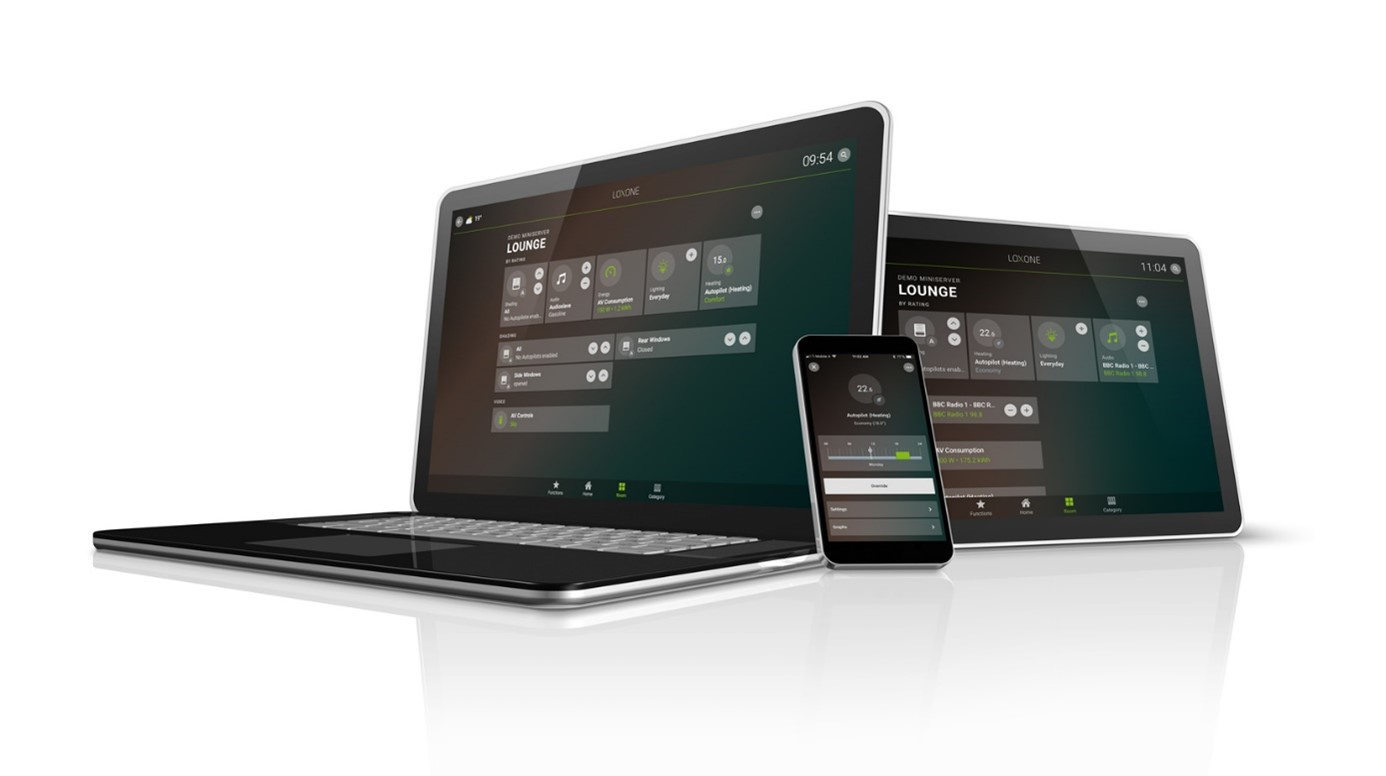
\includegraphics{obrazky/loxone-app.jpg}
	\caption{Loxone App. Převzato z Loxone web}
	\label{loxone-app}
\end{figure}

Loxone Extensions (rozšíření) slouží pro rozšíření funkcí Miniserveru. K Miniserveru se připojují pomocí sběrnice Loxone Link (kterou obsahují všechny verze Miniserveru). Tato sběrnice může být až 500 m dlouhá. Díky rozšířením může uživatel zakoupit systém pouze s těmi technologiemi, které chce opravdu využívat a nemusí tak platit za zbytečné vlastnosti systému. Příkladem rozšíření mohou být Tree Extension (pro připojení až 100 Tree zařízení; zejména pro doplnění Miniserveru 1. generace, který neobsahuje rozhraní pro komunikaci přes tree sběrnici) \cite{TreeDatasheet}, Air Base Extension (Pro doplnění Miniserverů 1. a 2. gen – k bezdrátové komunikaci) \cite{AirBaseExtensionDatasheet}, Dimmer Extension (pro stmívání světel) \cite{DimmerExtensionDatasheet} a mnoho dalších\footnote{https://shop.loxone.com/cscz/extensions.html}.

Loxone nabízí pro automatizaci domácnosti více než 400 produktů \cite{ReseniLoxone}.
Loxone pro propojení prvků v systému vyvinulo tzv. Loxone Tree technologii. Jedná se o sběrnici, na kterou je možné připojit až 50 prvků, a Loxone uvádí, že díky tomu je možné ušetřit až 80\% kabeláže. Podobně jako Loxone Link, i Loxone Tree může sahat až 500 m daleko.

V oblasti inteligentního vytápění nabízí Loxone souhru technologií pro vytápění, chlazení, rekuperaci, a automatizovanou stínící techniku, což přináší do regulace vytápění vysokou efektivitu \cite{RizeniKlimaLoxone}.

Z hlediska regulace teploty nabízí tzv. „zónové“ vytápění. Jedná se o inteligentní topení, které na rozdíl od klasického inteligentního vytápění (zahrnující obvykle nějaký bezdrátový termostat, Wi-Fi termostatické hlavice apod.) umožňuje inteligentněji řídit teplotu tím, že uživatel zvolí, ve které místnosti (případně i ve který čas) má být jaká teplota. Uživatel chytrého domu s tímto systémem si tak může navolit například větší teplo v koupelně oproti místnosti, kde spí. Tento systém tak umožňuje mít větší kontrolu nad vytápěnými místnostmi, potažmo vyšší efektivitu.

Inteligentní vytápění Loxone podporuje režim učení, systém se tedy na základě předchozích zkušeností spustí vytápění tak, aby byla v dané místnosti požadovaná teplota ve správný čas. Uživatel si tak může nastavit například to, aby měl v 7:00 vyhřátou koupelnu na 23 °C. \newline
Loxone vytápění má dle oficiálních stránek \cite{LoxoneRegulaceTeploty} následující výhodné vlastnosti:
\begin{itemize}
    \item Inteligentní řízení teploty – využití již zmíněného režimu učení k dosažení požadované teploty v žádaný čas. Loxone rovněž při regulaci zohledňuje venkovní teplotu.
    \item Úspora nákladů – Loxone dokáže inteligentně rozhodovat o nejefektivnějším řešení. Například energeticky náročnou klimatizaci může nahradit energeticky výhodnějším stínění
    \item Režim nepřítomnosti – systém od Loxone podporuje úsporný režim pro chvíle, kdy uživatel není doma
    \item Ochrana budovy – Loxone dokáže reagovat na různá nebezpečí, například v případně vzniku požáru vypnout ventilaci i rekuperaci
    \item Loxone aplikace a statistiky – Loxone nabízí zdarma aplikaci na zařízení s androidem, přes které uživatel může sledovat i nastavovat teplotu v domě vzdáleně
    \item Notifikace – v případě problému s některou technologií Loxone upozorní uživatele
    \item Státní svátky – na základě znalosti státních svátků může Loxone adekvátně upravovat svoji činnost
    \item Údržba – Loxone uživatele upozorňuje na termín pravidelné údržby
\end{itemize}
Z hlediska automatizace domácnosti v porovnání s dříve uvedenými systémy je rovněž důležitá přítomnost ovládané chytré zásuvky. Ta s Miniserverem komunikuje technologií Loxone Air. Má v sobě teplotní čidlo a rovněž elektroměr s vyhodnocením výkonu a spotřeby 

//TODO ještě zmínit loxone touch a tlačítko na stůl

\subsection*{Jablotron}
Jablotron je česká firma, která se od svého založení zaměřuje především na zabezpečovací systémy \cite{OJablotronu}. Kromě nich se také zabývá zabezpečením a monitoringem vozidel, topením a ventilací, monitoringem dechu a rovněž ovládáním a automatizací domácnosti \cite{NaseChytraReseniJablotron}.

Jablotron nabízí několik různých systémů. Dva nejnovější jsou Jablotron 100 a Jablotron 100+ \cite{OJablotronu}. Primárním úkolem obou systémů je zabezpečení budov, ovšem je možné je využít i v oblasti automatizace (zejména díky programovatelným výstupům). Samotné zabezpečení je možné využít v rámci automatizace (automatické zapnutí světel při odkódování alarmu) \cite{J100Manual}. Na své systémy poskytuje Jablotron při splnění podmínek až 7letou záruku\footnote{https://www.jablotron.com/cz/produkty/alarmy/alarm-do-domu/}.

Pro odjištění/zajištění systému se vždy musí provést nejprve autorizace uživatele. Systém totiž uchovává informaci o oprávnění jednotlivých uživatelů. Každému z uživatelů je možné pro účely autorizace přiřadit jeden kód (4, 6 nebo 8místný) a až dva RFID čipy \cite{J100Manual}. Funkce, které je možné v těchto systémech použít jsou:
 \begin{itemize}
     \item Zapínání a vypínání
     \item Akce v kalendáři (časovače)
     \item Automatické akce \cite{JLinkManual}
 \end{itemize}
Mezi akce, které lze automatizovat v systému Jablotron patří zejména ovládání světel, ovládání žaluzií, chytrá termoregulace (řízení vytápění a klimatizace) \cite{ChytraFirma} či ovládání jiných zařízení pomocí programovatelných výstupů. 

Systém od Jablotronu je možné rozdělit na tyto různé části:
\begin{itemize}
    \item Ústředna
    \item Různé vstupní či výstupní prvky
    \item Aplikace MyJablotron
    \item Program J-Link
\end{itemize}
Ústředna v systémech Jablotron slouží jako centrální prvek, který shromažďuje informace ze snímačů a patřičně na ně reaguje. Komunikace mezi prvky systému a ústřednou může probíhat podobně jako u systému Loxone buď pomocí kabelů, nebo bezdrátově. Zařízení, která komunikují pomocí kabelu se zde nazývají sběrnicové \cite{J100Manual}. Mezi produkty firmy Jablotron pro automatizaci domácnosti je možné najít:

\begin{itemize}
    \item Záplavový detektor
    \item Snímač teploty
    \item Magnetický detektor (detekce otevření dvěří/okna)
    \item Termoelektrická hlavice
    \item Relé na DIN lištu 
    \item a další\footnote{https://www.jablotron.com/cz/katalog-produktu/}
\end{itemize}

Systém Jablotron 100+ je možné ovládat celkem 4 způsoby, a to:
\begin{itemize}
    \item Přístupovým modulem
    \item Mobilní aplikací pro chytré telefony (MyJABLOTRON)
    \item Webovou aplikací (rovněž MyJABLOTRON)
    \item Či klíčenkou \cite{JablotronVasDum}
\end{itemize}

Přístupový modul slouží pro rychlé odjištění/zajištění objektu, případně k dalším funkcím automatizace. Jablotron nabízí celkem 3 typy těchto modulů:

\begin{itemize}
    \item Čtečka RFID karet
    \item Klávesnice se čtečkou RFID karet
    \item Klávesnice s displejem a čtečkou RFID karet
\end{itemize}

Ke každému z modulů je možné připojit až 20 segmentů. Ty obsahují popisek a dvě prosvětlená tlačítka. Jejich funkcí může být buďto zajištění/odjištění, signalizace stavu (například signalizace otevření garážových vrat) nebo ovládání zařízení v rámci automatizace (například žaluzií) \cite{J100Manual}. Barvy prosvětlení odpovídají semaforu, kde červená odpovídá stavům jako zajištěno/zapnuto, žlutá zajištěno částečně a zelená znamená odjištěno/vypnuto. \newline
Jak již bylo zmíněno, systém od Jablotronu lze ovládat rovněž mobilní aplikací MyJablotron. Je k dispozici jak na Google Play (pro zařízení s androidem), tak i na App Store (pro iOS zařízení). Kromě toho existuje i její webová verze. Jablotron tak nabízí rychlý přehled o tom co se děje v domácnosti. Ovládání domácnosti přes aplikaci funguje podobným způsobem jako přístupový modul – pomocí tlačítek s barvami semaforu.

Klíčenka k ovládání systému je dostupná ve dvou verzích – jednosměrný a obousměrný ovladač. Ten druhý má výhodu v tom, že provedení akce je potvrzeno kontrolkou na ovladači. V případě chyby tak ví, že je mimo dosah ústředny a akce se neprovedla \cite{J100Manual}.

K nastavení uživatelských parametrů v systému (jako oprávnění) slouží program J-Link. V něm je možné definovat uživatele i s jejich přístupovými oprávněními, provádět diagnostiku systému, kontrolu programovatelných výstupů a vytvářet či upravovat kalendář akcí (pro ovládání automatizovaných funkcí) \cite{JLinkManual}.

\subsection*{Apple HomeKit}
Apple HomeKit je systém, který umožňuje uživateli bezdrátově ovládat nejrůznější chytrá zařízení v domácnosti. Na rozdíl od systémů jako je Loxone je HomeKit orientován spíše na bezdrátovou komunikaci. V základu je sytém založen na komunikaci pomocí Wi-Fi a Bluetooth. Pro podporu dalších přenosových technologií je potřeba do systému přidat tzv. bridge, který potom slouží jako prostředník mezi zařízeními. Zařízení v systému mezi sebou komunikují pomocí aplikačního protokolu HAP. Pokud dané koncové zařízení tento protokol nezná, tak s ním komunikuje bridge zařízení pomocí protokolu, kterému rozumí, takže bridge opět funguje jako prostředník \cite{HomeKitChytraDomacnost}.  

Systém Apple HomeKit je možné ovládat pomocí chytrého telefonu iPhone. V tomto případě je však možné ovládání pouze v lokální síti. Druhou variantou je ovládání přes internet, ale to již vyžaduje použití nějakého bridge, tedy centrálního prvku (např. Apple TV či iPad). 
Pro ovládání systému pomocí telefonu s operačním systémem Android je potřeba mít v systému nějakého hlasového asistenta, který je se systémem Apple HomeKit kompatibilní (např. Amazon Alexa či Google Assistant) \cite{JakZacitHomeKit}.

Mezi zařízení, která je možné v systému Apple HomeKit používat patří např. nejrůznější tlačítka, světla, kamery, zásuvky a mnoho dalšího (viz. seznam na stránkách společnosti Apple\footnote{https://www.apple.com/ios/home/accessories/}). Systém Apple HomeKit představuje otevřený systém, do kterého postupně přibývají nové prvky, přičemž se nejedná jen o zařízení od společnosti Apple. Obchodníci s těmito zařízeními pak uvádějí u konkrétních zařízení, zda jsou s Apple HomeKit kompatibilní, pokud tak tomu je \cite{HomeKitDokonalost}.

Po přidání zařízení do systému (v aplikaci Domácnost) je možné zařízení ovládat jednak okamžitým nastavováním hodnoty \cite{StavimeChytrouDomacnostApple2}, ale také je možné využít automatizace, která umožňuje zakomponovat některou z následujících situací:
\begin{itemize}
    \item Někdo přijde 
    \item Někdo odejde
    \item Nastane určitá denní doba
    \item Změna stavu příslušenství
    \item Čidlo něco detekovalo \cite{StavimeChytrouDomacnostApple3}
\end{itemize}

Na zařízení s operačními systémy iOS, iPadOS, watchOS či macOS je možné je ovládat pomocí aplikace Domácnost\footnote{https://support.apple.com/cs-cz/guide/iphone/iph22d98bbca/ios}. Případně je také možné použít aplikaci Zkratky či ovládání pomoci hlasového asistentovi Siri \cite{StavimeChytrouDomacnostApple}. Nakonec je samozřejmě také možné jednotlivá chytrá zařízení ovládat pomocí aplikace od jejich dodavatele \cite{StavimeChytrouDomacnostApple2}.


\subsection*{Sonoff}
Sonoff je bla bla…


\subsection*{Home connect}
Poněkud jiný přístup k chytré domácnosti přináší technologie Home connect. Tou jsou vybavena některá zařízení, například od společnosti Bosh\footnote{https://www.bosch-home.com/cz/novinky/home-connect}. Předchozí zmíněné systémy slouží k ovládání a automatizaci spíše jednoduchých prvků domácnosti, jako jsou světla, zásuvky apod. Naproti tomu technologie Home connect je přítomna v některých spotřebičích, jako je například pračka, lednice či kávovar. Aplikace, která s Home connect přichází je dostupná na operační systém Android, ale také pro hlasové asistenty Amazon Alexa či Google Assitant. Díky aplikaci je možné získávat některé informace o spotřebičích (např. zda nejsou dveře lednice pootevřené) a také zařízení ovládat (např. na dálku zapnout troubu a předehřát ji tak) \cite{HomeConnect}.

\subsection*{Virtuální hlasoví asistenti a centrální prvky chytré domácnosti}
Virtuální osobní asistent (VPA) je osobní asistent, který zajišťuje interakci mezi uživatelem chytré domácnosti a zařízeními v ní. Jako jiné označení se rovněž používá inteligentní, digitální osobní, či mobilní asistent. Je-li ovládaný hlasem, pak se někdy označuje jako hlasový asistent \cite{TalkingToSmartDevices}. Dále v textu této kapitoly je vždy asistentem míněn právě hlasový asistent, nebude-li specifikováno jinak. Jedná se o software, jehož úlohou je asistovat uživateli při nejrůznějších příležitostech, mezi jinými i při ovládání domácnosti. Hlasoví asistenti běží na některém zařízení s reproduktorem a mikrofony nebo mobilním zařízení. Dnes jich existuje na trhu veliké množství (zejména pro chytré telefony). Mezi nejznámější představitele hlasových asistentů v současné době patří:
\begin{itemize}
\item Apple Siri
\item Amazon Alexa
\item Microsoft Cortana
\item Google Assistant \cite{VoiceAssistantsIntro}
\end{itemize}

Podobně jako systém Apple HomeKit mají obecně i hlasový asistenti (resp. zařízení, která je obsahují) funkci centrálních jednotek, které spojují jednotlivá zařízení. Při výběru chytrých zařízení pro automatizaci domácnosti je tedy vhodné se ujistit, zda podporuje daného hlasového asistenta\footnote{https://www.alza.cz/jak-postavit-chytrou-domacnost}.

V současné době žádný z výše uvedených hlasových systémů nepodporuje češtinu, nicméně Assistant od společnosti Google by ji v dohledné době mohl podporovat \cite{GoogleAssistantCestina}. Zřejmě i Siri bude brzy podporovat češtinu \cite{SiryCZ}. Amazon Alexa pak sice nerozumí česky, ale již dokáže číst některé knihy v češtině. Pro českého uživatele jsou tak pouze 2 možnosti – buďto používat asistenta v angličtině a spokojit se s případnou absencí některých funkcí, které nejsou v Česku podporované (například ovládání domácnosti), nebo použít některého českého virtuálního asistenta, ovšem s omezenou funkcionalitou oproti jejich vyvinutějším protějškům. Mezi české hlasové asistenty patří například:
\begin{itemize}
\item Emma
\item Intelli
\end{itemize}

Každý z virtuálních asistentů má své vlastní specifikace, ovšem jsou některé úlohy, které je možné považovat za typické:
\begin{itemize}
\item Číst a psát SMS a emailové zprávy, uskutečňovat hovory
\item Nastavovat časové a kalendářové akce (časovače, upomínky…)
\item Odpovídat na některé základní informativní otázky (počasí, čas, převody jednotek…)
\item Ovládat média jako televizi či připojené reproduktory (pouštět filmy, hudbu)
\item Vyprávět vtipy a příběhy
\item Konečně ovládat prvky chytré domácnosti \cite{VoiceAssistantsIntro}
\end{itemize}

Používání virtuálních osobních asistentů nejen, že umožňuje přistupovat k různým úkolům inovativním a interaktivním způsobem, ale v mnoha případech i zjednodušuje jinak relativně zdlouhavou činnost. Dobrým příkladem je manuální nastavení budíku (bez použití VPA). Na mobilním telefonu (Nexus 5) je dle \cite{TalkingToSmartDevices} potřeba vykonat následující akce:
\begin{enumerate}
\item Kliknout na tlačítko pro návrat na domovskou obrazovku (pokud se tam uživatel nenachází)
\item Kliknout na ikonu hodin
\item V otevřené aplikaci najít ikonu budíku a kliknout na ni 
\item Kliknout na tlačítko „+“ pro přidání budíku
\item Nastavit hodinu, překliknout na volbu minuty a nastavit minuty
\item Potvrdit kliknutím na tlačítko „OK“
\end{enumerate}
Při použití hlasového asistenta je celá úloha značně zredukována pouze na aktivování asistenta a vyslovení požadovaného úkolu.

Bez použití VPA je dokonce řada úkolů nerealizovatelná. Například připomenout či udělat něco v okamžiku, kdy se uživatel vrátí domů -- což je funkce, kterou někteří virtuální asistenti podporují \cite{CoJeSmartHomeHub}. Interaktivitu zajišťují virtuální asistenti i při automatizaci domácnosti, pro její řízení není potřeba otevírat k tomu určené (a mnohdy jednoúčelové) aplikace, ale stačí vyslovit žádost, třeba i s jistou vzdáleností od zařízení s hlasovým asistentem a ten se již o vše postará. Kromě toho v sobě virtuální asistenti mohou mít i funkce sloužící přímo pro automatizaci domácnosti. Například nastavení podmínek, scénářů atd.
Virtuální asistenti díky svým funkcím a vlastnostem k chytré domácnosti neodmyslitelně patří, ovšem je nutné si uvědomit, že zde nejsou nutností. Spíše často fungují jako prostředník mezi uživatelem a chytrými zařízeními, který usnadňuje řízení domácnosti. Často pak bývají zabudováni do chytrého zařízení, plnící funkci centrálního prvku (hubu), jako tomu je v případě zařízení Echo od společnosti Amazon. 

Emma je český hlasový asistent, kterého vytvořil David Beck pomocí aplikace Zkratky (na systému iOS). Jak již bylo zmíněno, nativním virtuálním asistentem pro iPhone je Siry, ta však zatím neumí česky, a to se rozhodl změnit David Beck\footnote{https://helloemma.cz/}. Nejedná se o samostatnou aplikaci, ale o zkratku v aplikaci Zkratky na systému iOS. Tato aplikace zkratky umožňuje uživatelům sloučit různé akce do jedné zkratky. Celkově pro zkratku Emma nastavil 7 tisíc akcí a další se chystá přidávat. Systém v současné době podporuje kromě češtiny 6 dalších jazyků \cite{HelloEmmaManual}.

\chapter{Protokoly a technologie používané v automatizované domácnosti}
Následující část je shrnutím protokolů a technologií, používaných systémy automatizace domácnosti. Není encyklopedickým výkladem problematiky, ale souhrnem informací, které mají k práci bezprostřední vztah. První část se věnuje protokolům CoAP a MQTT, jelikož se jedná o nejpoužívanější protokoly pro IoT. Následuje obecný úvod k technologii bezdrátového přenosu a nakonec uvádím krátké seznámení s technologiemi Wi-Fi, Bluetooth a ZigBee. Samotné technologii Wi-Fi je věnována samostatná podkapitola, jelikož je později využita v realizační části práce.

\section{Komunikační protokol CoAP}
CoAP protokol je protokol, určený pro komunikaci mezi uzly (zařízeními) s omezenými zdroji v omezené síti (tedy např. s vysokou ztrátovostí paketů). Je definován v RFC 7252\footnote{https://tools.ietf.org/html/rfc7252}. Tento protokol je speciálně navržený zejména pro tzv. machine-to-machine komunikaci v rámci internetu věcí. CoAP protokol se svojí strukturou podobá aplikačnímu protokolu HTTP, ačkoli každý z těchto protokolů má jiné zaměření. Mezi velkou výhodu CoAP protokolu patří jeho malá režije a jednoduchost \cite{CoAPStepByStep}.

\subsection*{Používané principy}
Jak už bylo zmíněno, tento protokol je velmi podobný protokolu HTTP. Podobně jako při komunikaci přes HTTP, i v CoAP existují 2 role, které zařízení může zastávat - klient a server. Klient posílá požadavek na server a ten vrací odpověď. Na rozdíl od HTTP je však při použití CoAP běžné, že zařízení vystupuje v obou rolích (vzhldem k povaze M2M interackce). V jednu chvíli tedy může zařízení jako klient posílat požadavky jinému zařízení a následně samo v roli serveru obsluhovat klienty.
Dalším rozdílem oproti HTTP je rovněž to, že se jedná o asynchronní protokol (používá UDP protokol). Z toho důvodu je nutné nějakým způsobem zaručit doručení dat (pokud je to pro danou aplikaci nutné). CoAP protokol proto definuje 4 typy zpráv:
\begin{itemize}
    \item Confirmable (potvrditelná)
    \item Non-confirmable (nepotvrditelná)
    \item Acknowledgment (potvrzení)
    \item Reset \cite{RFC7252}
\end{itemize}

Jelikož je CoAP protokol navržen pro ztrátovou síť, počítá se s jistými ztrátami jednotlivých zpráv. Protokol tedy rozlišuje mezi potvrditelnou a nepotvrditelnou zprávou. Pokud příjemce obdrží potvrditelnou zprávu, musí odpověďět zprávou typu acknowledgment (potvrzení). V případě, že vyprší časový limit a příjemce neobdrží tuto odpověď, znovu odešle původní zprávu. Toto provádí dokud není dosaženo maximálního počtu opakovaných přenosů \cite{CoAPCongestionControl}.Tento počet je definován dokumentem RFC 7252 v rámci přenosových parametrů a je roven číslu 4, ale je možné jej (spolu s ostatními parametry) upravit pro danou aplikaci. Odesílatel vyhodnotí případnou přijatou zprávu jako odpověď podle identifikátoru zprávy, který se posílá spolu se zprávou. Ten musí být v odpovědi stejný jako v původním požadavku. Pokud zařízení posílá nepotvrditelnou zprávu, neočekává se, že příjemce pošle zpět potvrzení. Zpráva typu reset se používá, pokud chce příjemce odesílateli sdělit, že potvrditelnou zprávu nedokáže zpracovat, resp. ani vrátit vhodnou chybovou odpověď \cite{RFC7252}.

\subsection*{Formát CoAP zprávy}
Formát CoAP zprávy je možné vidět na obr. \ref{coap-format}.
\begin{figure}[hbt]
	\centering
    \makebox[\textwidth]{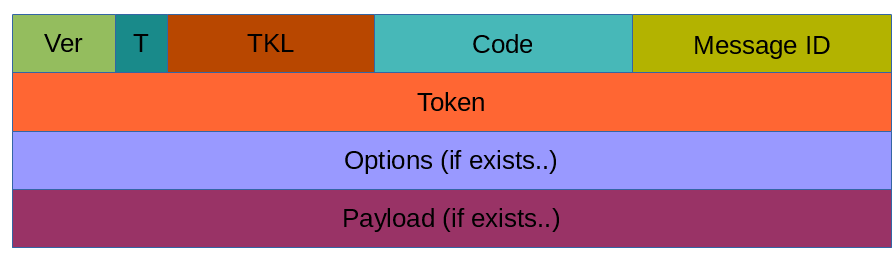
\includegraphics[width=\paperwidth/2]{obrazky/coap-format.png}}
	\caption{Formát CoAP zprávy\protect\footnotemark }
	\label{coap-format}
\end{figure}
 \footnotetext{https://www.survivingwithandroid.com/wp-content/uploads/2018/11/coap-message-format.png}
 
CoAP zpráva je zakódovaná pomocí binárních dat. Začíná povinnou 4-bitovou hlavičkou, obsahující informaci o:
\begin{itemize}
    \item Verzi CoAP protokolu (Ver) - 2 bity
    \item Typ zprávy - 2 bity
\end{itemize}
Verze protokolu musí být nastavena na 1 (zbylé možnosti jsou určeny pro budoucí verze protokolu). Typ zprávy je myšlen z hlediska potvrditelnosti, jak bylo definováno výše. Jednotlivým hodnotám odpovídají následující typy:
\begin{itemize}
    \item 0 - confirmable (potvrditelná)
    \item 1 - non-confirmable (nepotvrditelná)
    \item 2 - acknowledgment (potvrzení)
    \item 3 - reset
\end{itemize}

Po typu zprávy je ve zprávě specifikována délka přítomného tokenu (4 bity). Na základě této délky může mít token 0-8 bajtů (délka 9-15 je rezervnována a nesmí být nastavená). Následuje kód zprávy, kterým může být buď metoda požadavku (CoAP je totiž podobně jako HTTP postaven na REST \cite{CoAPCongestionControl2} architektuře), nebo stavový kód odpovědi, který má opět podobný účel jako stavové kódy u HTTP protokolu. Tento kód má délku 8 bitů. Poslední součástí hlavičky CoAP zprávy je identifikátor zprávy, který má délku 16 bitů. Používá se k identifikaci duplikátních zpráv a rovněž ke spojení potvrditelné zprávy s potvrzením (resp. reset zprávou). 
Po hlavičce následuje token, který má delku 0-8 bajtů, jak bylo vysvětleno dříve. Tento token se používá ke spojení požadavku a odpověďi. Při komunikaci totiž může odesílatel poslat požadavek na server, na který sice může server ihned odpovědět potvrzením (zde tedy posílá stejný identifikátor zprávy, jaký měl požadavek), ale daný požadavek vyřeší až později. A tehdy posílá server klientovi stejný token, jako obdržel v původní zprávě od klienta, ačkoli identifikátor zprávy již bude jiný. To je tedy rozdíl mezi identifikátorem a tokenem.
Po tokenu následují tzv. options, tedy volby, které mají podobnou funkci, jako některé hlavičky v HTTP protokolu. Tyto volby mohou mít různou délku a rovněž jejich počet může být různý (ani nemusejí být přítomny).
Poslední částí CoAP zprávy tvoří nepovinný datový obsah (payload).

\section{MQTT protokol}
MQTT (Message Queuing Telemetry Transport protokol) je aplikační protokol, určený podobně jako CoAP pro přenos dat v nestabilní síti. Narozdíl od CoAP se však nejedná o protokol typu klient -- server, ale používá tzv. publish--subscribe mechanismus \cite{AutomaMQTT}. Jednotlivé uzly v síti mohou tedy mít jednu ze tří funkcí:
\begin{itemize}
    \item Publisher
    \item Subscriber
    \item MQTT broker
\end{itemize}
\subsection*{Publish--subscribe mechanismus}
Mechanismus publish--subscribe je založen na tom, že v systému existují zařízení, která sdílí nějaké údaje (publish). V síti je přítomen MQTT broker, což je zařízení, které má funkci centrálního prvku, přes který se odehrává komunikace. 
Pokud chce nějaké zařízení naslouchat novým informacím od jiného zařízení, musí se (u brokeru) přihlásit k odběru jeho zpráv. Stane se tak z něj subscriber daných zpráv. Identifikace zařízení (resp. zpráv), kterým bude naslouchat se pak provádí přes tzv. topic (téma). To specifikuje cestu k danému zdroji a má hierarchickou strukturu. Může mít podobu například "domov/kuchyně/světlo". Jelikož jsou témata v MQTT zprávě zakódovány v UTF-8, mohou používat dokonce diakritiku.
Pokud naopak nějaké zařízení potřebuje naslouchat na změny od nějakého zařízení, přihlásí se u brokeru k odběru daných zpráv, které opět specifikuje cestou, na které bude naslouchat.
Pokud následně zařízení typu publisher získá nějaký údaj, který sdílí (např. hodnotu měřené veličiny), odešle zprávu MQTT brokeru. Ten zprávu přepošle všem zařízením, které jsou přihlášeny k odběru daného tématu.
Jedno zařízení může samozřejmě vystupovat pro určitá témata jako publisher a pro jiná jako subscriber \cite{RootMQTT}.

\subsection*{Quality of Service}
Jelikož je protokol určen pro funkci i v nestabilní síti, definuje 3 stupně tzv. QoS (Quality of Service):
\begin{itemize}
    \item 0 - At most once
    \item 1  - At least once
    \item 2 - Exactly once \cite{IoTQoS}
\end{itemize}

Stupeň 0 říká, že odesílatel zprávu odešle a zahodí, nekontroluje tedy, zda zprávu přijali příjemci. V podstatě se jedná o obdobu nepotvrditelné zprávy u CoAP protokolu.
Stupeň 2 rozhoduje, že odesílatel po odeslání zprávy čeká na potvrzení od příjemce, že zprávu dostal. V případě, že vyprší stanovený časový limit a toto potvrzení neobdrží, tak zprávu odesílá znovu.
Poslední stupeň se používá, pokud chce mít odesílatel jistotu, že příjemce dostal (resp. zpracoval) zprávu přesně jednou. K tomuto účelu se používá čtveřice zpráv. Nejprve odesílatel posílá sdílená data. Následně čeká na potvrzení. Pokud od příjemce nepřijde potvrzení, posílá zprávu znovu se značkou, definující, že se jedná o duplicitní zprávu. Po přijetí potvrzení posílá příjemci další zprávu jako potvrzení, že obdržel potvrzení. Nakonec příjemce posílá zpět zprávu pro potvrzení, že byl přenos dat úspěšně dokončen \cite{HiveMQ}.

\section{Bezdrátový přenos dat a signálů}
Pro přenos dat či řídících signálů je vždy potřeba zvolit vhodné médium, přes které se budou tyto informace přenášet. V některých situacích není pro přenos vhodné (a někdy dokonce ani možné) používat kabely (ať už metalické nebo optické). V těchto případech je potřeba přenášet informace bezdrátově, tj. za využití jiných médií, jako je vzduch. 
Podobně jako je nutné u kabelového spojení využít vhodný způsob komunikace (například zvolit vhodnou sběrnici a nastavit ji správné parametry) je potřeba se způsobem komunikace zabývat rovněž u bezdrátového přenosu. Zde je nutné zejména zvolit vhodnou technologii (jako je Wi-Fi, Bluetooth či ZigBee) a její parametry \cite{4technologie}.

\subsection*{Výhody bezdrátového přenosu}
Bezdrátová komunikace má oproti kabelové řadu výhod. Zejména se jedná o následující:

\begin{itemize}
    \item Jednodušší připojení – zařízení není potřeba připojovat kabelem, a dokonce nemusí být ani vybaveno konektorem pro toto připojení (pozn. pro dálkový přenos prostřednictvím světla je však stále potřeba mít nějaký přijímající port). Z toho rovněž plyne, že není potřeba měnit strukturu sítě kvůli změnám v místnosti a rovněž není potřeba myslet na konkrétní strukturu sítě ještě před budováním.
    \item Větší spolehlivost – častým zdrojem problémů s kabelovým připojením jsou chyby na straně kabelů – jejich poškození. Použitím bezdrátových technologií se lze vyhnout tomuto typu chyb.
    \item Snadná rozšiřitelnost sítě – u kabelového připojení je potřeba řešit způsob rozšíření sítě a v případě, že stávající struktura sítě rozšíření nepodporuje, tak je potřeba ji celou pozměnit. Bezdrátové sítě tento problém eliminují.
    \item Nižší cena – použitím bezdrátových technologií se značně sníží pořizovací cena sítě – není potřeba kupovat drahou kabeláž. Rovněž instalace kabelů do starých budov může být velmi nákladná a problémová.
\end{itemize}

\subsection*{Nevýhody bezdrátového přenosu}
Kromě množství výhod, které bezdrátová komunikace představuje jsou zde rovněž některé nevýhody tohoto typu komunikace:

\begin{itemize}
    \item Rušení signálu – zařízení, využívající bezdrátové technologie, může způsobovat rušení ostatních zařízení a rovněž opačně – dané zařízení může být rušeno od ostatních zařízení, pracujících na podobném principu
    \item Bezpečnost – bezdrátová komunikace často vysílá (a přijímá) signály do relativně rozsáhlého otevřeného prostoru, tudíž jsou takto vysílaná data často daleko méně chráněná než u kabelového přenosu (kde je k získávání dat potřeba mít fyzické připojení k síti, ve které se data přenáší) \cite{wirelessComunication}. Je tedy nutné zabezpečit přenos dat.
\end{itemize}

\section{Technologie bezdrátového přenosu Wi-Fi}

Wi-Fi je technologie, využívající standardů z rodiny IEEE 802.11. První verze tohoto standardu byla organizací IEEE schválena v roce 1977 \cite{4technologie}. Od té doby vyšlo mnoho dalších verzí standardů. Jednotlivé verze se od sebe mohou odlišovat různými parametry, například frekvenčním pásmem, šířkou pásma jednotlivých kanálů, maximální rychlostí přenosu apod. Organizace Wi-Fi Alliance rozlišuje některé standardy IEEE 802.11 číslem generace Wi-Fi, nejnovější je zatím 6. generace, oznámena byla již i 7 \cite{WiFi7}. 

\begin{figure}[hbt]
	\centering
	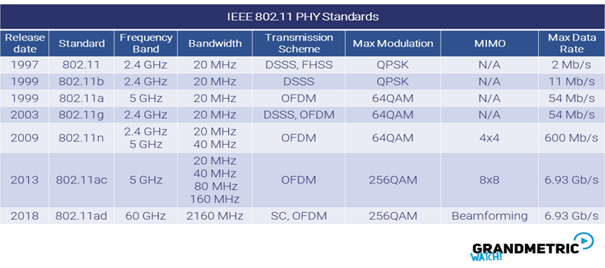
\includegraphics[scale=0.95]{obrazky/wifi-standards.png}
	\caption{Některé důležité verze standardu IEEE 802.11 a jejich parametry. Převzato z \url{https://www.grandmetric.com/2018/05/29/wi-fi-standards-evolution/}}
	\label{wifi-standards}
\end{figure}
Wi-Fi funguje na principu vysílání a přijímání rádiových vln. Organizace IEEE rozhodla využít pro technologii Wi-Fi frekvence z ISM\footnote{ISM -- Nelicencované frekvenční pásmo pro průmysl, vědu a lékařství (industrial, scientific and medical)} pásma \cite{BezdratoveSite}. Wi-Fi standardně využívá frekvencí 2,4 GHz a 5 GHz. Nejprve byla zařízení Wi-Fi schopná pracovat pouze v jednom z těchto dvou frekvenčních pásem, ale 4. generace (IEEE 802.11n) přidává možnost práce v obou zmíněných pásmech. Moderní zařízení s Wi-Fi si tak mohou vybrat (a dokonce během své činnosti měnit) frekvenci, na které budou spolu komunikovat.
Obě pásma mají svá pro i proti. Mezi výhody pásma 2,4 GHz patří zejména větší pokrytí signálu a rovněž větší kompatibilita (platí spíše pro starší zařízení). Na druhou stranu pásmo 5 GHz nabízí podstatně vyšší přenosové rychlosti a dále větší množství komunikačních kanálů \cite{WifiFrequencyBands}. Wi-Fi generace 6E a připravovaná gererace 7 umožňuje komunikaci i na frekvenci 6 GHz \cite{WiFi7}.

\subsection*{Režim sítě}
Wi-Fi nachází uplatnění v (bezdrátových) lokálních sítích. V nich pak rozlišujeme 3 režimy na základě toho, jak se Wi-Fi zařízení v síti mezi sebou navzájem spojují (jakou plní roli):
\begin{itemize}
    \item Režim infrastruktury
    \item Ad hoc režim
    \item Smíšený režim
\end{itemize}

V režimu infrastruktury je v sítí přítomen minimálně jeden centrální prvek (tzv. přístupový bod), který zprostředkovává komunikaci mezi jednotlivými prvky (klienty) sítě, případně poskytuje připojení do jiné sítě přes distribuční systém (DS). V tomto režimu sítě je výhoda, že je snadné připojit do stávající infrastruktury nový prvek. \newline
Ad hoc je režim bezdrátové sítě, ve které není přítomen žádný centrální prvek (přístupový bod), se kterým by prvky sítě komunikovali, ani zde není žádné spojení s pevnou sítí přes distribuční systém. Jedná se tedy o decentralizovanou síť. Jednotlivé prvky tedy mezi sebou navzájem komunikují přímo (toto spojení se někdy označuje jako tzv. peer-to-peer). V tomto režimu má síť rovněž SSID identifikátor, kterým je možné síť identifikovat \cite{BezdratoveSite}

\section{Ostatní technologie bezdrátového přenosu}
\subsection*{Technologie Bluetooth}
Bluetooth je standard, definovaný v IEEE 802.15.1. Vytvořila jej firma Ericsson v roce 1994 a od té doby vyšlo několik nových verzí \cite{4technologie}. Podobně jako Wi-Fi pracuje v ISM pásmu 2,4 GHz. Na rozdíl od Wi-Fi však není definován pouze na prvních dvou vrstvách ISO/OSI, ale definuje protokoly na všech sedmi vrstvách tohoto modelu. Na nejnižší úrovni, kde definuje způsob přenosu jednotlivých bitů využívá metodu FHSS, která zajišťuje, že při přenosu bitů vysílač přeskakuje mezi několika frekvencemi \cite{GettingStartedBluetooth}.

Zařízením, které jej využívají, umožňuje vytvořit tzv. PAN (osobní síť). V těchto sítích má každé zařízení přiřazeno unikátní 48bitovou adresu BD\_ADDR (BlueTooth Device Address) -- jedná se o obdobu MAC adresy u ethernetu. Tu používá pro komunikaci s ostatními zařízeními. Jedno zařízení může být v roli master (řídící), slave (podřízená) nebo obojího \cite{BluetoothGuide}. K jedné řídící stanici se připojuje jedno a více podřízených zařízení (používá se pouze adhoc komunikace mezi master a slave stanicí). Zde hovoříme o tzv. piconetu (pikosíti). Maximální počet zařízení v jedné pikosíti je 8 (jedna řídící stanice a až 7 podřízených). Stanice náležící do jedné pikosítě může zároveň patřit do jiné pikosítě. Jedná se tedy o rozšíření sítě mezi zařízeními. Takto vytvořenou síť nazýváme tzv. scatternet (rozprostřená síť). V každé rozprostřené síti má každá pikosíť unikátní identifikátor – je jím BD\_ADDR její řídící stanice. Díky rozlišení jednotlivých pikosítí pak může každá tato síť využívat jiné skokové sekvence (frekvenčních kanálů, na kterých se vysílají/přijímají data) \cite{WirelessPersonalCommunications}. Výhodou Bluetooth technologie je její nízká spotřeba energie (zejména od verze 4) \cite{IoTProtocols}.

\subsection*{Technologie ZigBee}
Zigbee je bezdrátová technologie, založená na standardu IEEE 802.15.4. Je určená pro vytváření sítě PAN (osobní síť) a pracuje v pásmu ISM 868 MHz, 902-928 MHz a 2,4 GHz \cite{4technologie}. 

ZigBee standard specifikuje 2 typy zařízení – FFL (Full Function Device) a RFD (Reduced Function Device). FFL zařízení je obvykle schopné mnoha funkcí a je stále aktivní, zatímco RFD se nachází většinu času v režimu spánku, ze kterého se občas probudí, například aby odeslalo hodnoty neměřené na nějakém senzoru.

V síti pak každé ze zařízení plní některou ze 3 funkcí:
\begin{itemize}
    \item Koordinátor
    \item Koncové zařízení
    \item Směrovač
\end{itemize}

Na základě definovaných zařízení pak existují 3 možné topologie ZigBee sítě:
\begin{itemize}
    \item Hvězda
    \item Strom
    \item Mesh síť \cite{HandsOnZigBee}
\end{itemize}

ZigBee podobně jako Bluetooth definuje komunikaci na všech úrovních modelu ISO/OSI, nekopíruje však přesně jednotlivé vrstvy. První 3 vrstvy modelů ISO/OSI a ZigBee si odpovídají, ale vrstvy L4-L7 jsou spojené do vrstev APS (Application Support) a ZDO (ZigBee Device Object) \cite{ZigbeeWirelessNetworking}.
TODO: Thread, WeMo, ZigBee and Z-Wave (https://www.tomsguide.com/us/smart-home-wireless-network-primer,news-21085.html)

\chapter{Vestavné systémy}
\label{vestavne-systemy}
Následující část je shrnutím současného stavu v oblasti vestavných systémů. Není encyklopedickým výkladem problematiky, ale souhrnem informací, které mají k práci bezprostřední vztah. Nejprve je zde úvod do vestavných systému, mikropočítačů a mikrokontrolerů. Následně je pojednáno o platformě Raspberry Pi, modulech ESP8266 a ESP32 a nakonec o možnostech, jaké se nabízejí pro bezdrátovou komunikaci popsaných zařízení.

\section{Vestavné systémy, mikropočítače a mikrokontrolery}

Vestavný systém můžeme definovat jako software spolu s počítačem, zabudovaným do nějakého zařízení takovým způsobem, že jej uživatel nevidí jako počítač \cite{DesigningEmbeddedSystems}. Tento počítač je většinou jednoúčelový, určený pro předem navržené použití. Tím se liší od univerzálních počítačů, které mohou poskytovat různé funkce a jejichž uplatnění se může měnit (jako je tomu u osobního počítače) \cite{EmbeddedSystems}.

Mezi hlavní charakteristiky vestavných systémů patří:
\begin{itemize}
    \item Jsou jednoúčelné - vestavné systémy jsou navrženy pro konkrétní účel a ten se v průběhu jejich funkce nemění
    \item Jsou na ně kladena omezení - při návrhu vestavných systémů se klade důraz zvláště na parametry jako jsou cena, velikost, spotřeba energie a výkon tak, aby měl výsledný systém ideální poměr těchto parametrů
    \item Reakce v reálném čase - spousta vestavných systémů musí neustále kontrolovat změny prostředí, pro které byly navržené a musí na ně v reálném čase odpovídat
    \item Jsou založené na mikroprocesorech či mikrokontrolérech
    \item Mívají připojené vstupní a výstupní zařízení
\end{itemize}
 Vestavný systém může buďto fungovat sám o sobě, nebo být součástí jiného systému \cite{ESOverview}.


\subsection*{Architektura vestavných systémů}
Složitost jednotlivých vestavných systémů se mezi sebou liší, nicméně většina z těchto systémů je tvořena 3 částmi:
\begin{itemize}
    \item Hardware -- jedná se o součásti systému jako je mikroprocesor, paměti apod.
    \item Software -- program, který vestavný systém vykonává
    \item RTOS -- real-time operační systém definuje, jakým způsobem systém funguje. U jednodušších systémů nemusí být přítomen
\end{itemize}

Z hlediska hardwaru je vestavný systém složen z následujících komponent:
\begin{itemize}
    \item Snímače -- převádějí snímaná fyzická data na elektrický signál
    \item Analogově-digitální převodníky -- převádějí analogový elektrický signál na digitální
    \item Procesor - zpracovává snímaná data a ukládá je do paměti
    \item Digitálně-analogové převodníky - převádějí digitální signál z procesoru na analogový
    \item Akční členy - převádějí výstupní data na výstupní akci \cite{ESArchitecture}
\end{itemize}

Z pohledu práce s daty pak můžeme typicky vestavné systémy rozdělit na ty, které využívají jednu z následujících architektur:
\begin{itemize}
    \item Von Neumannova architektura
    \item Harvardská architektura
\end{itemize}

Hlavním rozdílem je způsob práce s pamětí. Ve Von Neumannově architektuře je paměť pro program i data spojená do jedné paměti. To potom znamená, že procesor v jeden okamžik buď čte instrukci z paměti, nebo provádí operaci čtení/zapisování s daty.
v Harvardské architektuře je pak paměť pro program a data rozdělena na dvě samostatné, což znamená, že procesor může současně načítat instrukci z paměti i používat paměť pro operaci s daty \cite{ESOverview}.
Dále také existuje modifikovaná Harvardská architektura. Systémy, které ji využívají mají pro data i program společnou paměť, ale dvě různé sběrnice a oddělené cache paměti (do kterých si data a instrukce ukládají ze společné paměti) \cite{ModifiedHarvard}.

\begin{figure}[hbt]
	\centering
	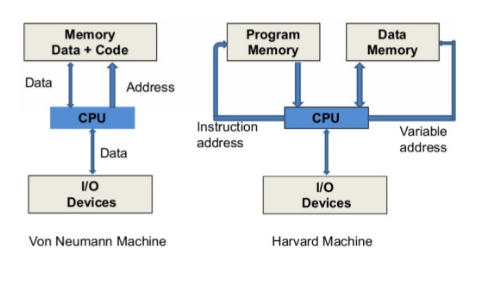
\includegraphics{obrazky/architektura-pocitace.png}
	\caption{Porovnání Von Neumannovy a Hardvarské architektury. Převzato z \url{https://vivadifferences.com/5-major-difference-between-von-neumann-and-harvard-architecture/}}
	\label{von-neuman-hardvard}
\end{figure}

Systémy, zahrnující mikroprocesory jsou obvykle založeny na Von Neumannově architektuře. Naopak systémy založené na mikrokontrolérech využívají Hardvarskou architekturu \cite{uCvsCPU}.

\subsection*{Mikroprocesor a mikrokontrolér}
Mikroprocesor (CPU) je programovatelné elektronické výpočetní zařízení, určené pro všestranné použití. Jedná se o čip, obsahující 3 základní součásti:
\begin{itemize}
    \item aritmeticko-logickou jednotku (ALU\footnote{ALU -- arithmetic logic unit})
    \item registry
    \item řídící jednotku
    \item sběrnici \cite{MicroprocessorAndInterfaces}
\end{itemize}

Mikroprocesor sám o sobě je z hlediska vestavěných systémů relativně jednoduché zařízení, které pro funkci systému potřebuje připojit některé další součásti, jako jsou paměti (RAM a ROM), čítače, časovač apod. Návrhář tedy musí tyto součásti přidat externě, aby zařízení fungovalo správně. 

Mikrokontrolér je zařízení, které na rozdíl od mikroprocesoru má již všechny součásti, potřebné pro svoji činnost v sobě. Obvykle však mívá mnohem nižší výkon než mikroprocesor \cite{uCvsCPU}.

\section{Jednodeskový počítač Raspberry Pi}
Raspberry Pi je levný univerzální počítač malých rozměrů. Poskytuje široké možnosti v oblasti multimédií a 3D grafiky, předpokládá se, že bude časem využíván i jako herní platforma \cite{RPiPrirucka}.  

\subsection*{Historie}
Raspberry Pi vzniklo v r. 2006 za přispění studijního ředitele pro informatiku na Cambridgeské univerzitě za účelem lokálních potřeb. Měl to být nástroj, který by poskytl prvotní impuls studentů k nějakému z univerzitních kurzů \cite{RPiPrirucka}. Vytvořil jej univerzitní profesor Eben Upton. V roce 2009 založil nadaci Raspberry Pi Foundation pro budoucí vývoj Raspberry Pi. Jeho cílem bylo vyvinout levný počítač, na kterém by se mladí studenti mohli učit programovat. Výsledkem byl počítač s cenou okolo 30ti dolarů, který měl školám pomoci ve výuce výpočetní techniky. Raspberry Pi se pak pro širokou veřejnost začalo prodávat oficiálně v únoru roku 2012 \cite{RPiBeginning}.

\subsection*{Verze a modely Raspberry Pi}
Jak již bylo zmíněno, při návrhu Raspberry Pi bylo přihlíženo zejména k ceně. Z tohoto důvodu hned u první oficiální verze vznikly 2 modely -- A a B. Model B měl být výkonnější (a tedy dražší) variantou modelu A. Verze 1, model B měl následující výbavu:
\begin{itemize}
    \item CPU -- 700Mhz ARM procesor
    \item RAM -- 512MB
    \item 2 USB porty
    \item HDMI, RCA Audio a SD slot
    \item 10/100 Ethernet
    \item 8 GPIO pins
\end{itemize}
Model A měl poloviční RAM paměť a jen jeden USB port \cite{RPiBeginning}. Od prvního vydání Raspberry Pi již vyšlo mnoho dalších verzí. Aktuálně nejvýkonnější verzí je 4, která nabízí je osazena čtyřjádrovým procesorem Cortex-A72 (1,5 GHz) a v závislosti na modelu je dostupná s RAM pamětí až 8GB\footnote{https://www.raspberrypi.org/products/raspberry-pi-4-model-b/specifications/}.

\begin{figure}[hbt]
	\centering
    \makebox[\textwidth]{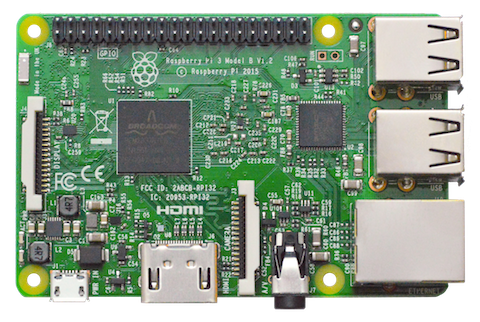
\includegraphics[scale=0.75]{obrazky/rpi3.png}}
	\caption{Raspberry Pi, verze 3B. Převzato z \url{https://developer.android.com/things/hardware/raspberrypi}}
	\label{rpi3}
\end{figure}

Níže je uveden seznam některých zajímavých parametrů Raspberry Pi verze 3B+, jelikož je tato verze použita v realizační části práce:
\begin{itemize}
    \item Čtyřjádrový procesor Cortex-A53 s frekvencí 
    \item 1GB LPDDR2 SDRAM
    \item HDMI
    \item 4 USB porty (verze 2.0)
    \item Wi-Fi a Bluetooth\footnote{https://www.raspberrypi.org/products/raspberry-pi-3-model-b-plus/}
\end{itemize}
Kromě těchto jednodeskových počítačů vydala nadace Raspebrry Pi Foundation verzi Pico. Jedná se o mikrokontrolér (bez OS) \cite{RPiP}.
\subsection*{Operační systém}
Na každou z verzí Raspberry Pi (kromě Pico) je možné nainstalovat některý z operačních systémů. Oficiálně podporovaným OS ze strany Raspebrry Pi Foundation je Raspberry Pi OS (dříve známý jako Raspbian)\footnote{https://www.raspberrypi.org/software/}. Ten obsahuje některé předinstalované nástroje jako internetový prohlížeč (Chromium). Existuje několik verzí tohoto OS \cite{RPiOS}.

\subsection*{Alternativy k Raspberri Pi}
Přestože má Raspberry Pi za sebou úspěšný vývoj a jedná se o jednu z nepopulárnějších plaforem, na trhu samozřejmě existují alternativní počítače. Někteří uživatelé mohou vyžadovat vyšší výkon, nižší cenu nebo některou kombinaci parametrů, kterou Raspberry Pi nenabízí. Mezi některé ze známějších alternativních jednodeskových počítačů patří:
\begin{itemize}
    \item ASUS Tinker Board S
    \item Banana Pi M64
    \item Odroid-XU4
\end{itemize}
Jednotlivé jednodeskové počítače se mezi sebou liší různými parametry jako je velikost a typ paměti RAM, použitý procesor, vstupní a výstupní porty, podporované OS \cite{RPiAlternatives} apod.

\section{Moduly společnosti Espressif Systems a alternativní mikrokontroléry}
Jak bylo uvedeno v úvodu této kapitoly, vestavné systémy mohou být mj. založeny na mikrokontrolérech. Mikrokontrolérů je dnes na trhu celá řada a vzájemně se mezi sebou liší množstvím různých parametrů. Pro snazší vývoj se mohou jednotlivé mikrokontroléry zabudovat do tzv. vývojových desek (někdy také pod pojmem vývojových kitů), které pak usnadňují přístup k GPIO, sběrnicím a usnadňují nahrávání nového kódu do daného mikrokontroléru \cite{DevKit}.

\subsection*{Espressif Systems}
Moduly ESP od společnosti Espressif Systems patří mezi jedny z nejznámějších mikrokontrolérů. Vyznačují se nízkou cenou, Wi-Fi stackem a schopností provozu RTOS\footnote{RTOS - Realtime-operating system (real-time operační systém)}. Existují již celkem 4 řady (generace) těchto čipů:
\begin{itemize}
    \item ESP8266
    \item ESP32
    \item ESP32-S2
    \item ESP32-C3
\end{itemize}
Všechny moduly obsahují 32bitový mikroprocesor. Na obrázku \ref{ESP-srovnani} je možné vidět porovnání vlastností prvních dvou řad modulů (ESP8266 a ESP32):
\begin{figure}[hbt]
	\centering
	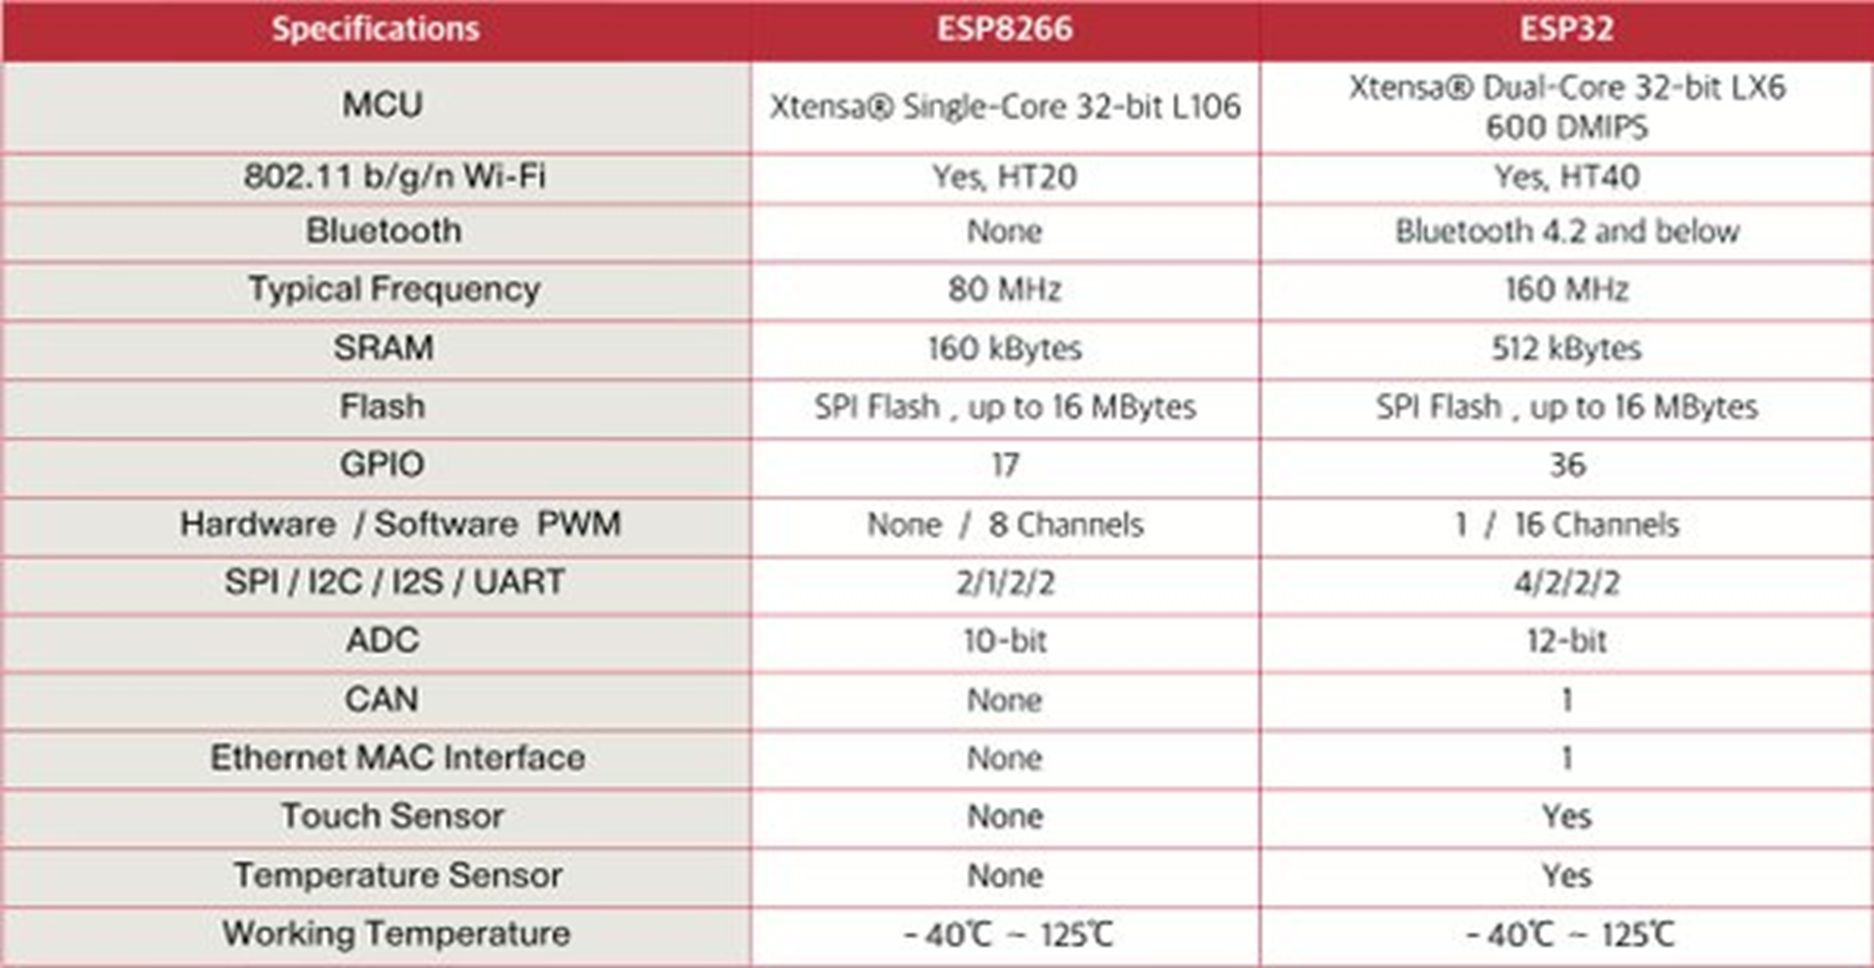
\includegraphics{obrazky/ESP.png}
	\caption{Srovnání specifikace modulů ESP8266 a ESP32. Převzato z \url{https://www.cnx-software.com/2016/03/25/esp8266-and-esp32-differences-in-one-single-table/}}
	\label{ESP-srovnani}
\end{figure}

Jednotlivé řady se mezi sebou liší některými vylepšeními, zejména v oblasti bezpečnosti a dále výkonem. Řady ESP32 a ESP32-C3 těchto mikrokontrolérů obsahují rovněž Bluetooth\footnote{https://www.espressif.com/en/products/modules}.

ESP moduly se prodávají jednak jako samostatné čipy, ale je možné je zakoupit i jako přídavný komunikační modul k jinému mikrokontroléru\footnote{https://dratek.cz/arduino/910-tcp-ip-wifi-modul.html}. Také je možné je pořídit jako součást vývojové desky. Mezi nejznámější vývojové desky s ESP8266 moduly patří ESP-01, Lua NodeMcu a WeMos D1 Mini \cite{BestESP}.

\subsection*{Ostatní mikrokontrolery a vývojové desky}
Mezi nejznámější vývojové desky patří Arduino. Jedná se o platformu využívající převážně 8-mi bitové mikrokontrolery. Její součástí je C/C++ framework (založený na programovacím jazyce Wiring) a IDE\footnote{IDE -- Integrated Development Environment (Vývojové prostředí)} pro snadný vývoj. Nejznámější varianta Arduino Uno obsahuje mikrokontrolér ATmega328, má 14 digitálních vstupně/výstupních pinů (z toho 6 s možností PWM modulace) a 6 analogových vstupních pinů. K vývojovým deskám Arduino vzniklo mnoho klonů. Pro možnost komunikace přes Wi-Fi je nutné buď využít verzi Arduino s Wi-Fi čipem, nebo dokoupit tzv. WiFi shield\footnote{https://store.arduino.cc/arduino-wifi-shield}. Nutno dodat, že cena Arduina se zmíněným Wi-Fi čipem/shieldem mnohokrát převyšuje dříve zmíněné moduly ESP. Arduino s Wi-Fi čipem je možné koupit na českém trhu za cenu okolo 1300 Kč\footnote{https://www.alza.cz/arduino-uno-wifi-rev2-d5655517.htm}, zatímco vývojová deska s ESP8266 Lua NodeMcu stojí okolo 150ti Kč\footnote{https://www.laskarduino.cz/iot-esp8266-lua-nodemcu-v2-wifi-modul--tcp-ip/}.

Jako alternativy Arduino vývojových desek je obecně možné považovat různé klony Arduina, kterých je opravdu velké množství. Často mají tyto vývojové desky i odvozený název, jako je Seeeduino\footnote{https://www.seeedstudio.com/Seeeduino-V4-2-p-2517.html}, Freeduino\footnote{https://freeduino.org/freeduino\_open\_designs.html} apod. Vybrané platformy ESP a Arduino mají velkou podporu mezi uživateli, jsou relativně levné a snadno dostupné. Vývojových desek (resp. mikrokontrolérů) však samozřejmě existuje velké množství, ale zmíněné patří mezi nejznámější.

\chapter{Zhodnocení současného stavu a plán práce}
V této kapitole se věnuji zhodnocení již existujících řešení automatizace domácnosti. Následně uvádím můj návrh řešení na základě nastudovaných řešení a vhodného rozsahu práce. Nakonec v bodech stanovuji cíle vyplývající z návrhu řešení, které se v práci snažím splnit.
\section{Zhodnocení současného stavu v oblasti automatizace domácnosti}

Na trhu se v současné době nachází velké množství systémů. Z těch, které jsem popsal v části o existujících řešení, je nejrozvinutějším systémem ten od společnosti Loxone. Zabírá opravdu širokou škálu možností a jen stěží by se hledala aplikace, pro kterou by nebyl vhodný (z hlediska automatizace). Kromě komplexnosti u něj oceňuji rovněž českou jazykovou lokalizaci. V češtině je k dispozici jak aplikace na ovládání (Loxone App), tak rovněž program pro konfiguraci systému (Loxone Config). Čím mě Loxone mile překvapilo je, že jsem si jejich aplikaci Loxone App mohl vyzkoušet v demoverzi i bez zakoupených komponent.

Jako nevýhodu Loxone vidím příliš vysokou cenu. Uživatel, který si chce nainstalovat pár chytrých zařízení, bude zřejmě překvapen cenou. Například při pořízení 3 chytrých zásuvek a miniserveru (který je k ovládání zásuvek potřebný) zaplatí přibližně 15 000 kč. Přitom adekvátní řešení od jiných firem, jako sonoff bude stát necelé 3000 kč, což je velký rozdíl – a při rozšiřování domácnosti o další prvky tento rozdíl znatelně roste. Na druhou stranu, pokud uživatel staví nový dům, může řešení od Loxone stát srovnatelnou cenu, jako konkurenční „neinteligentní“ instalace. Jako další nevýhodu vidím to, že celkově je instalace systému orientovaná spíše pro profesionální montáž pro pracovníky s příslušnou klasifikací (většina produktů je určena k zabudování do rozvaděče, příp. ke komunikaci s moduly v něm). Celkově je však řešení od Loxone na hodně vysoké úrovni.

Řešení od firmy Jablotron je jistě zajímavé jejich dvoutlačítkovými (rozšiřitelnými) segmenty. Zdá se mi však nepraktické spojovat přístupovou klávesnici do domu s prvky automatizace domácnosti. Působí to poněkud omezeně. Navíc rozhraní pro ovládání domácnosti a alarmu v aplikaci MyJablotron se snaží napodobovat onu klávesnici, což příliš k přehlednosti nepřispívá. Na druhou stranu pro uživatele, jehož hlavní požadavek je zabezpečení objektu a pouze doplňková automatizace domácnosti (jako rozsvícení světel při odjištění domu), budou systémy od firmy Jablotron ideální. Cenově pak toto řešení vychází nepatrně levněji\footnote{https://www.lupa.cz/clanky/zabezpecovaci-zarizeni-jablotron-100-co-nabizi-a-co-umi/}, než Loxone (ale vždy samozřejmě záleží na volených komponentách, které uživatel vyžaduje). Pokud však není vyžadováno zabezpečení domácnosti (ale pouze automatizace světel) pak je toto řešení celkem drahé. Zajímavou možností však je spojení obou zmíněných systémů, které je možné díky převodníku JA-121T (https://www.loxone.com/cscz/blog/bezpecny-chytry-dum-od-jednicek-na-trhu/).

Systém HomeKit je zajímavý v tom, že zde není potřeba žádný „speciální“ centrální prvek – pokud již uživatel vlastní například iPad (či jiný produkt, který zastoupí funkci centrálního prvku). Samozřejmě pokud takový prvek v domácnosti shání, tak se jeho pořízení stává další investicí. Co je ale na systému HomeKit pozitivní, je jeho nízká cena ve srovnání se systémy od společnosti Loxone či Jablotron. Systém HomeKit se stále rozrůstá a má velkou podporu v rozmanitosti produktů. A na rozdíl od předchozích zmíněných systémů je více orientovaný na běžné uživatele (v tom smyslu že nevyžaduje montáž od specialistu). Jednou z nevýhod je zde to, že je systém orientovaný zejména na bezdrátovou komunikaci, která samozřejmě někdy může být méně spolehlivá. Tím spíše, že mnoho produktů komunikuje pouze pomocí Bluetooth, takže si uživatelé musejí hlídat dosah zařízení. Obecně se však jedná o cenově dostupnou variantu chytré domácnosti.

\begin{figure}[hbt]
	\centering
	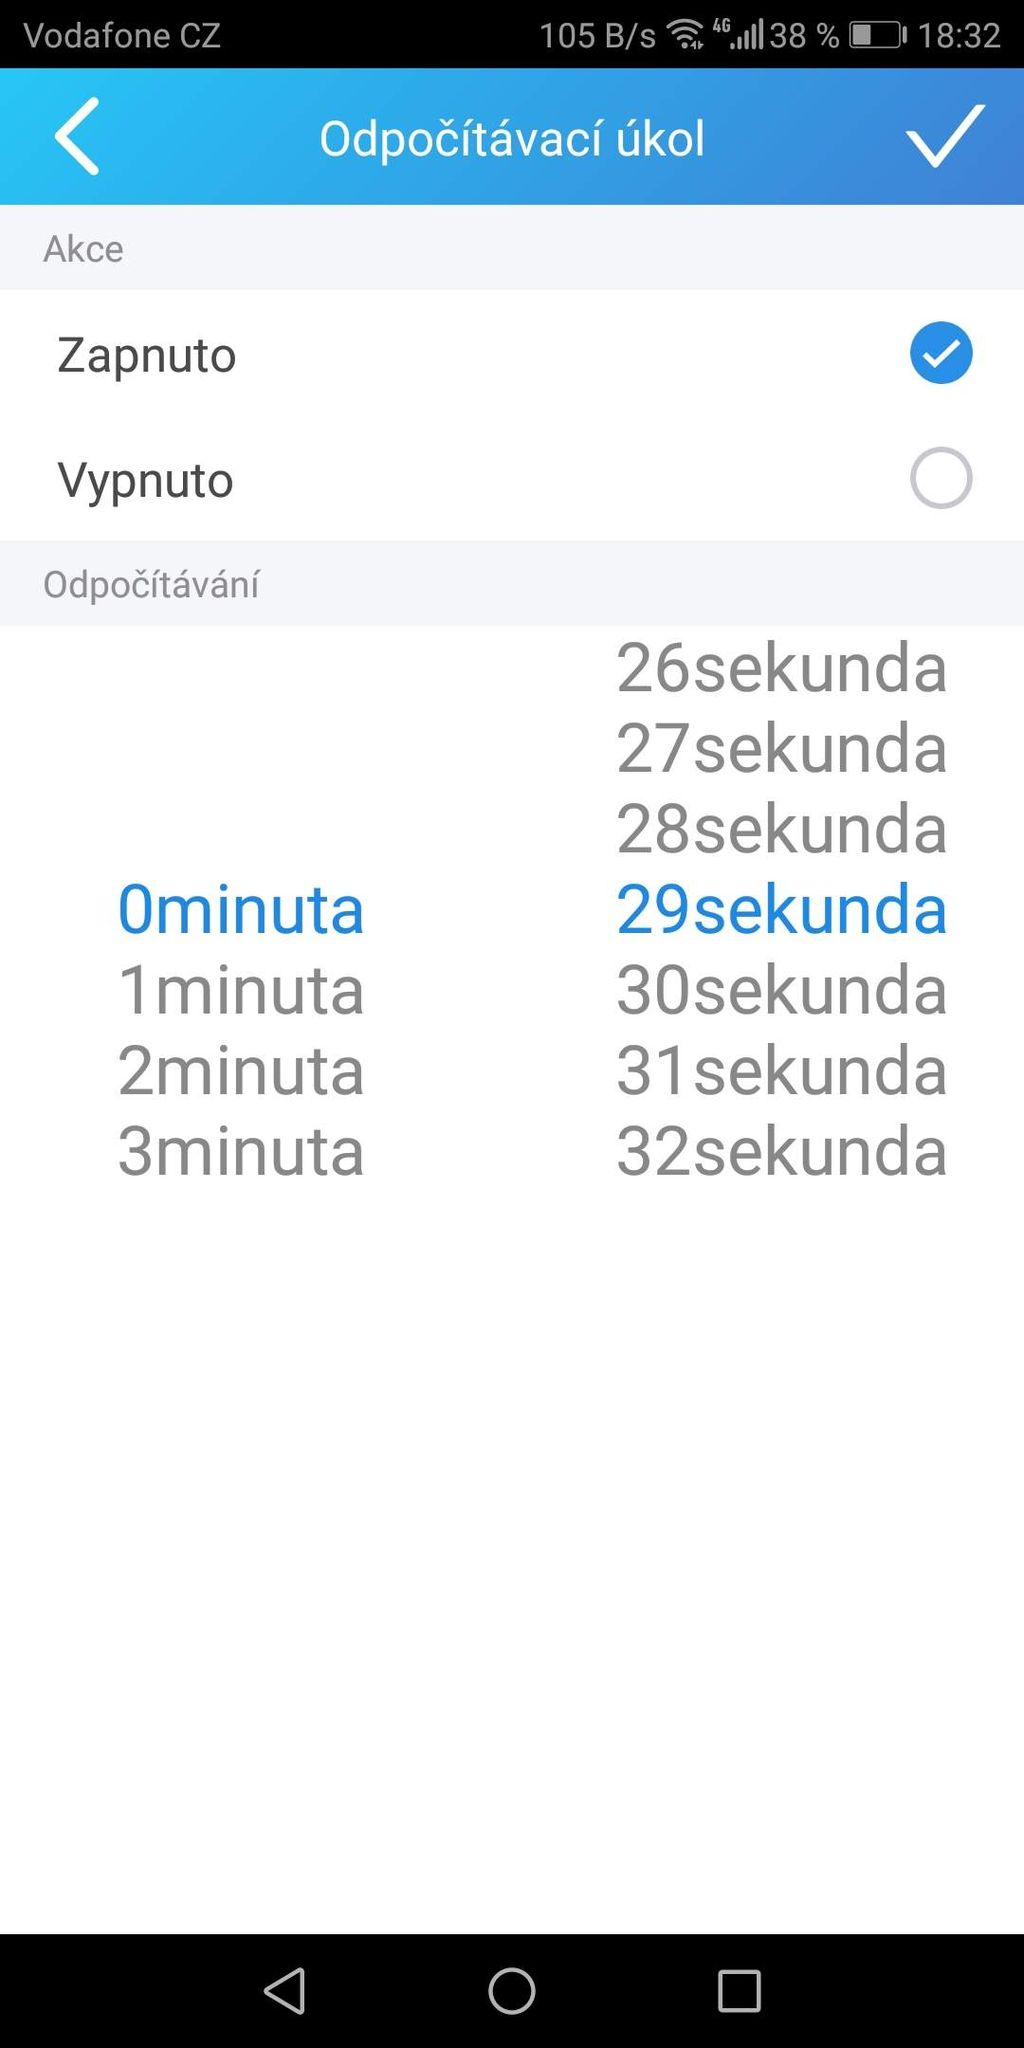
\includegraphics[scale=0.15]{obrazky/kangtai.jpg}
	\caption{Ukázka nastavení časovače pro Wi-Fi zásuvku Kangtai. Maximální doba nastavení je 59 minut a 59 vteřin. Pro každé zařízení je možné mít v jednu chvíli nastavený pouze jeden takový časovač. Vlastní obrázek.}
	\label{kangtai}
\end{figure}

Systémy Sonoff a Kangtai pak nabízejí podobné možnosti, jako HomeKit a i cena je srovnatelná. Je tedy možné na ně pohlížet jako na alternativy. Samotné řešení od společnosti Kangtai jsem sám vyzkoušel (v podobě Wi-Fi zásuvky). Všeobecně se jedná o spolehlivé zařízení, výtky mám pouze k jejich aplikaci. V starší aplikaci\footnote{https://play.google.com/store/apps/details?id=com.bugull.kangtai} určené k ovládání zásuvky, která byla uvedena v přiloženém manuálu jako výchozí\footnote{https://www.tipa.eu/en/smart-wifi-socket-kangtai-51062/d-175329/} se mi podle manuálu nepodařilo nové zařízení do systému přidat. Nová aplikace\footnote{https://play.google.com/store/apps/details?id=com.ktapp.wifi} je na tom lépe (přidání zařízení proběhlo bez problému), ale má některé menší nedostatky.

Zejména není možné spustit více časovačů na jednom zařízení současně. Nový časovač je možné nastavit vždy až po vypršení předchozího. Kromě toho aplikace nezobrazuje přívětivým způsobem zbývající čas, kdy k nastavené akci dojde. Jediná možnost jak jej zobrazit je otevřít nastavení časovače (jakoby uživatel chtěl nastavit nový), kde uvidí zbývající čas ve vstupu, kde případný nový čas nastavuje, viz obrázek \ref{kangtai}. Tento způsob ale považuji za neintuitivní (navíc pro aktualizaci zbývajícího času je potřeba se vrátit zpět a opět vstoupit do časovače). 

Problémovým je i maximální doba, kterou jde na časovači nastavit, která činí méně než hodinu. Také některým uživatelům může vadit absence snímačů (alespoň jejich zobrazování v oficiální aplikaci), ale jelikož je možné systém propojit s některými virtuálními hlasovými asistenty, tak podpora snímačů ze strany výrobce není nezbytná. Další věc, která se jeví jako nepříjemná je, že systém sám nedokáže rozpoznat, zda se uživatel nachází v lokální síti (a v případě chybějícího připojení k internetu přepnout systém na lokální funkci). Toto přepnutí je nutné provést manuálně a vyžaduje odhlášení z uživatelského účtu.

Systém HomeConnect vnáší do automatizace domácnosti zajímavý koncept. Zatímco některé systémy umožňuji automatizovat domácnosti například chytrými zásuvkami či spínači, HomeConnect ve spolupráci s jinými společnostmi vyvíjí přímo spotřebiče s prvky chytré domácnosti, čímž tyto spotřebiče obsahují mnohem více „inteligence“, na rozdíl od pouhého „zapínání/vypínání“. Nicméně nevýhodou je zde příliš malý sortiment produktů, a tudíž jednoúčelová aplikace navíc, kterou stejně musejí uživatelé doplnit o další aplikace, chtějí-li například rovněž ovládat zásuvky, světla či rolety. Kromě toho je rovněž cena produktů dost vysoká.

\section{Návrh technického řešení}
Na základě výzkumu dostupných řešení a jejich zhodnocení jsem se rozhodl vyvinout systém, který bude mít některé základní prvky automatizace. Svými funkcemi se bude podobat řešení jako je Sonoff či Kangtai, ale chtěl bych vyřešit některé nedostatky, se kterými jsem se u Wi-Fi zásuvek společnosti Kangtai setkal. Především bych chtěl přidat možnost více současných časovačů, přehlednější zobrazování zbývajícího času a také možnost automatizace na základě snímačů. Také bych chtěl implementovat intuitivnější rozlišování zda je ovládající zařízení v lokální síti, nebo zda ovládá systém přes internet. 
Základem práce tedy bude především dálkové ovládání jednoho zařízení druhým, (jelikož je to zadání mé bakalářské práce). V systému tedy bude figurovat nějaký ovladač a dále ovládané prvky. 

V práci bude nutné zvolit vhodné vestavné zařízení, které bude sloužit jako server a také zařízení, která budou přijímat povely od tohoto serveru. Zde končí podobnost s popsanými systémy Sonoff či Kangtai, protože jsem se rozhodl, že ovládaný prvek zde nebude žádné konkrétní zařízení (jako zásuvka či lampička) ale spíše obecný modul se vstupně-výstupními porty, přes které bude možné ovládat jiná, už konkrétnější zařízení. Pro plnohodnotnou funkci systému bude tento modul nutné opatřit dalšími přídavnými součástkami. Půjde zejména o relé pro možnost ovládání zapnutí a vypnutí zařízení připojeného k tomuto modulu (tímto způsobem bude možné například ovládat LED pásek, či vytvořit bezdrátovou zásuvku). K modulu budou připojeny rovněž tranzistory pro možnost použití PWM (pulzně šířkové modulace) na výstupech modulů -- takový výstup pak bude sloužit pro stmívání světel, zejména LED pásku či bodových LED světel na 12 V. Díky navrženým vlastnostem bude samozřejmě možné jednotlivé moduly zabudovat i jako součást jiných zařízení a ty tak doplnit o dálkové ovládání.

Aby bylo ovládání systému co nejjednodušší, bude zde možnost ovládání na dotykovém displeji. Ovládání systému jen z jednoho místa však není v oblasti automatizace úplně nejlepším a efektivním řešením (například uživatel sice nemusí dojít k vypínači světla, aby zhasl, ale stejně musí dojít někam k ovládacímu zařízení systému). Rozhodl jsem se tedy, že bude možnost ovládání i z telefonu, počítače a dalších zařízení (požadavky na zařízení budou definovaná později v podkapitole \ref{navrh-systemu}). 
Kromě přímého ovládání bude systém podporovat několik typů snímačů. Ty budou sloužit jednak pro informaci uživatele (o teplotě, vlhkosti vzhuchu apod.), ale bude možné je využít i při automatizaci (nastavit na určitou úroveň jas LED pásku, pokud intenzita venkovního světla klesne pod určitou úroveň či zapnout světlo při detekci osoby snímačem pohybu). Tyto automatizace bude možné libovolně zapínat a vypínat. Mezi snímači, které bude systém podporovat budou:

\begin{itemize}
    \item teploty
    \item vlhkosti vzduchu
    \item tlaku vzduchu
    \item intenzity světla
    \item pohybu
    \item sepnutí (kontaktu/tlačítka)
\end{itemize}

Jde o typické představitele analogových i digitálních senzorů. Pro účely práce budou použity jen tyto, nicméně řešení chci pojmout jako open source (a s ohledem na tento fakt se budu snažit o co největší rozšiřitelnost systému), a další snímače bude možné přidat v budoucnu.

Nakonec bude také možné výstupy ovládat pomocí nastavených časovačů, jak již bylo naznačeno. Jednotlivé časovače bude možné také zapínat a vypínat podle potřeby.


Mým řešením bych chtěl doplnit existující open source řešení o takové, které bude svými vlastnostmi určeno spíše pro nadšence v oblasti elektroniky a bude obsahovat českou jazykovou lokalizaci. Bude poskytovat jednoduchý systém pro ovládání mnoha zařízení pomocí jednoho vestavného zařízení s připojeným displejem. Svou prací bych si chtěl rovněž vyzkoušet celý návrh a realizaci systému automatizace domácnosti, který bych následně mohl sám využívat. U modulů s výhodou využiji, že budou mít více vstupů/výstupů a jeden modul tak může sdružovat více různých funkcí (mít připojeno několik snímačů a výstupních zařízení, místo jednoho). To bude také jistým vylepšením oproti některým již existujícím systémům. Také bych chtěl klást důraz zejména na nízkou cenu, která by u pár ovládaných zařízení (bez ceny těchto koncových zařízení) neměla přesáhnout 2000 kč.

Při práci budu využívat již existující moduly a mikropočítač (který bude sloužit jako „mozek“ systému), které však naprogramuji a vhodným způsobem doplním o některé elektronické součástky (jako zmíněné relé, či tranzistor). Práce se však nebude zabývat detailním konstrukčním návrhem prvků systému, ani návrhem DPS pro jednotlivé části hotového systému. Pro případné propojení součástek a zařízení systému budou použita nepájivá kontaktní pole.

\section{Požadované vlastnosti navrhovaného systému}
\label{navrh-reseni}
Na základě předchozích úvah jsem se rozhodl, že vytvořím systém, který bude splňovat následující vlastnosti:
\begin{itemize}
    \item Bude zvolen vhodný mikropočítač, který bude sloužit jako server
    \item k tomuto mikropočítači bude zvolen dotykový displej vhodných rozměrů, aby byl systém přehledný a mohl sloužit pro ovládání zařízení
    \item Displej by měl být rovněž vybrán s ohledem na možnost zobrazení přehledu o stavu zařízení v systému (zobrazení, která zařízení jsou zapnutá, či jaké hodnoty se nacházejí na PWM výstupu)
    \item k implementaci bude zvolen vhodný programovací jazyk
    \item bude podporována funkce přímého ovládání výstupů ovládaných modulů
    \item také zde bude funkce zobrazení dat ze senzorů
    \item systém bude obsahovat českou jazykovou lokalizaci
    \item v systému budou figurovat uživatelské účty, přičemž z jednoho účtu bude možné ovládat jen jednu domácnost
    \item bude zvolena vhodná technologie bezdrátového přenosu tak, aby byl systém co nejjednodušší na implementaci a případné rozšiřování
    \item projekt bude uvolněn jako open source, čímž bude cena systému jako takového pro potenciální uživatele minimální (daná pouze cenou použitých součástek a zařízení) a uživatelé se budou moci sami upravovat
    \item součástky a zařízení budou v systému voleny s ohledem na co nejnižší cenu
\end{itemize}

\chapter{Realizace a testování}
V této kapitole se věnuji vlastní realizaci řešení a následnému testování a vyhodnocení. V první podkapitole uvádím celkový návrh systému - tedy z jakých aplikací a zařízení se bude skládat, jak mezi sebou budou komunikovat apod. Následně se věnuji návrhu grafického uživatelského rozhraní pro aplikaci, přes kterou bude uživatel systém ovládat. Dále vysvětluji jakým způsobem se v systému ukládají data a jak jsem vyřešil autentizaci uživatelů. V dalších podkapitolách již rozebírám implementaci konkrétních aplikací. Nejprve klientské aplikace a v samostatné podkapitole dále popisuji spolu aplikaci pro Raspberry Pi a moduly ESP8266 (jelikož tyto dvě aplikace spolu přímo komunikují a jsou na sobě závislé). Nakonec uvádím jak jsem systém testoval a k jakým výsledkům jsem došel.

\section{Celkový návrh systému}
\label{navrh-systemu}
Systémy chytré domácnosti bývají různě komplexní a obvykle se skládají z různých zařízení a také aplikací (i když uživatel přímo přistupuje obvykle pouze k jedné hlavní s grafickým uživatelským rozhraním). Stejně tomu tak je v systému, který jsem navrhl já. Celkem jsou zde 3 (v různé míře) spolupracující aplikace a několik typů zařízení. Každé z těchto zařízení a aplikací zde má svou nezastupitelnou úlohu. Na obrázku \ref{architektura} je možné vidět celkovou koncepci systému. 

\begin{figure}[!hbt]
	\centering
	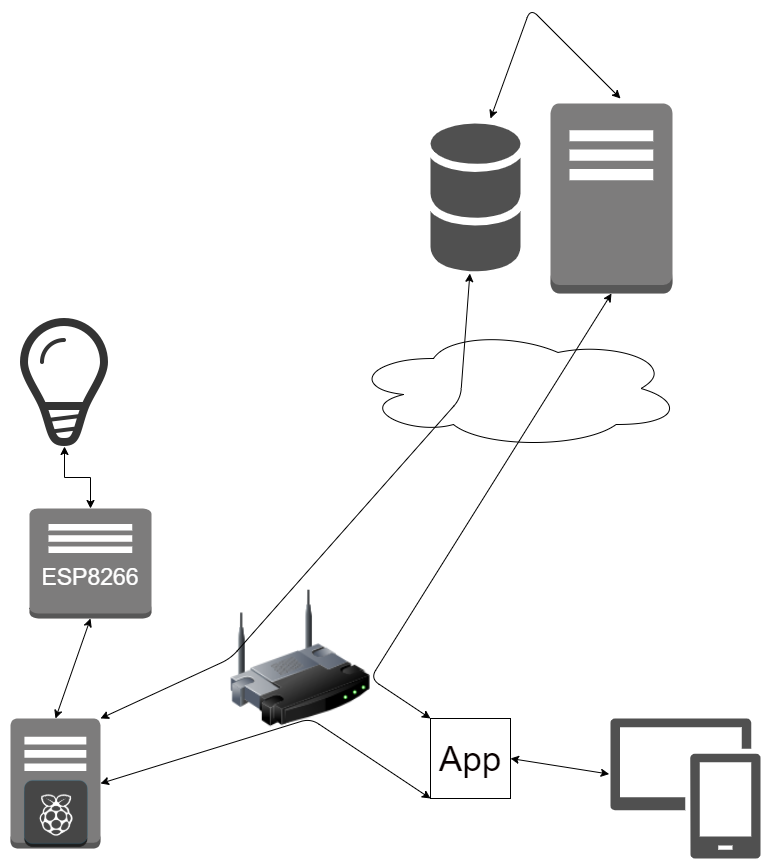
\includegraphics[scale=0.4]{obrazky/navrh-architektura.png}
	\caption{Architektura systému pro automatizaci domácnosti}
	\label{architektura}
\end{figure}

Pro uživatele jsou zde klíčovými různá zařízení s displejem (notebook, mobilní telefon, Raspberry Pi s displejem apod.), přes která může systém konfigurovat, ovládat a přes který je informován o naměřených hodnotách na snímačích. Prostřednictvím grafické aplikace na těchto zařízeních vlastně komunikuje s databází, resp. lokálním serverem. Jedná se vlastně o webovou aplikaci, kterou klientům zprostředkovává webový server (ať již přístupný na internetu přes webhosting, tak i lokální server). 

Jak je naznačeno na obrázku, v systému se nacházejí dvě databáze. Jedna z nich je přístupná v síti internet. Aby však bylo minimalizováno riziko napadení systému, tak má databáze nastavená přístupová pravidla (takže uživatel může přistupovat pouze k datům, která mu patří). Kromě toho je veškerá komunikace s databází zabezpečena pomoci protokolu SSL\footnote{Secure Sockets Layer}. Druhá databáze je uložená v lokálním serveru. Obě databáze by v ideálním stavu měli být v synchronizaci, ovšem nemusí tomu tak někdy být, zejména v důsledku odpojení lokálního serveru od internetu.

Lokální server má v systému za úkol nejen poskytovat webovou aplikaci, ale také funguje jako řídící jednotka. Naslouchá změnám ve vzdálené databázi a pokud k nějakým dojde, tak na ně patřičným způsobem reaguje (např. odešle pokyn k nastavení výstupu na některém koncovém modulu). Tímto způsobem je vyřešeno dálkové ovládání mimo lokální síť a samotná klientská zařízení (jako telefon) při přístupu přes internet nenavazují přímo s lokálním serverem žádnou komunikaci. Tyto změny ve vzdálené databázi se provádějí ve webové aplikaci na adrese \url{https://automatizace.web.app/}. Opačná situace nastává při připojení klientských zařízení k lokálnímu webovému serveru (tedy v lokální síti). V tomto případě webová aplikace nekomunikuje se vzdálenou databází, ale veškeré požadavky posílá na tento server. Ten následně požadavky zpracovává, změny ukládá do své lokální databáze a v případě potřeby (a připojení k internetu) je promítá do vzdálené databáze.

Dalším zařízením v systému jsou výstupní moduly. Ty mohou mít ke svým vstupům připojeny snímače a k výstupům pomocné součástky (jako relé či tranzistory) a k nim dále již výstupní ovládaná zařízení, jako jsou světla.

\subsection*{Zařízení a aplikace v systémů}
Jak tedy vyplývá z předchozího popisu koncepce systému, budou v systému tato zařízení:
\begin{itemize}
    \item server či řídící jednotka (s připojeným displejem)
    \item koncové moduly
    \item snímače
    \item ovládaná zařízení
    \item ostatní zařízení, přes která bude možné systém ovládat (klientská zařízení)
\end{itemize}

Server má na starosti řízení celého systému, jedná se tedy o centrální řídící jednotku. Pokud například uživatel zadá pokyn ke změně hodnoty na některém výstupu modulu, bude to právě tento server, který žádost zpracuje a pošle ji dále jako příkaz na konkrétní koncový modul. 
Jelikož bylo potřeba dle navrženého řešení v části \ref{navrh-reseni} připojit k centrální jednotce (dotykový) displej, musel jsem vybrat vhodný mikropočítač (protože mikrokontrolery mívají obecně daleko menší výkon) opatřený portem pro přenos obrazového signálu. Jedním z nejpoužívanějších mikropočítačů je Raspberry Pi. Je relativně levný (ve verzi 3B+ se dá sehnat okolo 1000 Kč, verzi Zero W je dokonce možné na českém trhu sehnat za přibližně 300 Kč) a tedy i snadno dostupný. Nadto je použití Raspberry Pi doporučeno v zadání mé práce. Pro účely bakalářské práce jsem tedy použil právě zmíněnou verzi 3B+. 

Koncový modul (dále již jen modul) je zařízení, které má vstupy a výstupy. Modul mění hodnoty na svých výstupech dle instrukcí, přicházejících ze serveru (Rapsberry Pi). K těmto výstupů pak mohou být dále připojeny příslušné součástky (jako relé či tranzistor) a k nim dále již reálná zařízení, ve kterých budou nějakým způsobem spínat kontakt. Může se tedy jednat o prosté zapnutí/vypnutí zařízení, jednoduché stmívání (PWM modulací na výstupu), ale také o pokročilé ovládání při zabudování tohoto modulu do nějakých dalších zařízení. Příkladem by mohla být řídící jednotka k ovládání žaluzií, která by na základě hodnoty na svém vstupu patřičným způsobem nastavila žaluzie. Tento vstup by poskytoval právě koncový modul (na svém výstupu). Jedná se však o příklad a v rámci bakalářské práce nic takového realizováno nebylo.
Moduly rovněž v pravidelných intervalech čtou hodnoty na svých vstupech (ke kterým jsou připojeny snímače). Jako modul bylo potřeba vybrat zařízení s nízkou cenou, jelikož těchto zařízení má být v systému obecně více. Kromě toho má modul přijímat pouze jednoduché instrukce od serveru, může se tedy klidně jednat o nějaký mikrokontrolér s omezeným výpočetním výkonem. Je však potřeba, aby byl schopný komunikovat po síti (tento požadavek vyplývá ze zadání mé bakalářské práce). Buďto bylo možné vybrat nějaký mikrokontrolér a k němu připojit modul, který jej o funkci komunikace po síti doplní (například vývojovou desku Arduino s WiFi shieldem), nebo zvolit takový, který již v sobě obsahuje prostředky nutné k bezdrátové komunikaci. Já jsem se rozhodl pro druhou možnost. Na trhu existuje spoustu takových mikrokontrolerů a vývojových desek, mezi nejznámější a zároveň nejlevnější patří ESP8266. Jelikož má pro danou aplikaci dostatečný výpočetní výkon, tak jsem použil právě tento modul.

Jako snímače jsem pro demonstraci vybral následující:
\begin{itemize}
    \item BMP280 (snímač tlaku a teploty)
    \item SHT21 (snímač teploty a vlhkosti)
    \item BH1750 (snímač intenzity světla)
    \item HC -- SR501 (PIR pohybové čidlo)
    \item tlačítko
\end{itemize}
Samozřejmě na trhu se nachází mnohem více nejrůznějších snímačů. Některé snímače pak vyžadují zvláštní konfiguraci (např. přepočet hodnoty). Proto jsem pro účely práce vybral těchto několik, které reprezentují základní snímače, které by uživatel v systému mohl chtít využívat. Samozřejmě bude možné v budoucnu systém rozšířit o nové typy snímačů.

Ovládanými zařízeními zde myslím ta, která budou připojena na výstup relé či tranzistoru, připojeného na některý z výstupů modulu. Jde tedy například o LED pásek či zařízení, u kterého se bude spínat nějaký kontakt. 

Klientská zařízení jsou libovolná zařízení s displejem, přes která bude uživatel moci ovládat systém. Jedinými požadavky na tato zařízení jsou zde vzhledem k implementaci (viz dále) následující:
\begin{itemize}
    \item schopnost komunikace pomocí Wi-Fi
    \item displej s dostatečnou uhlopříčkou (ideálně 5´´ a více) a rozlišením
    \item některý z podporovaných internetových prohlížečů, viz část \ref{provedene-testy} 
\end{itemize}

Samozřejmě zařízení samotná nestačí a aby systém nějakým způsobem fungoval, bylo potřeba pro některé jeho části vyvinout aplikace. Celkově jsou v systému aplikace 3:
\begin{itemize}
    \item aplikace s grafickým rozhraním
    \item server
    \item aplikace pro moduly
\end{itemize}

Aplikace s grafickým rozhraním je určena pro internetový prohlížeč na klientských zařízeních. Právě přes tuto aplikaci je možné celý systém ovládat a konfigurovat (z pohledu uživatele). 
Server běží na Raspberry Pi a od aplikace s grafickým rozhraním získává instrukce a vykonává je. Na základě těchto instrukcí server dále komunikuje s jednotlivými moduly.
Poslední aplikace je spuštěna na modulech. Jejím úkolem bude ovládat své výstupy na základě pokynů od serveru. Rovněž aplikace v pravidelných intervalech serveru posílá naměřené hodnoty od připojených senzorů.

Kromě těchto třech aplikací bude součástí systému (i když nepřímou) rovněž vzdálený webový server a vzdálená databáze. Nebudou sice nějakým způsobem umístěny fyzicky u uživatele (že by si je musel nějak pořizovat), nicméně jedná se rovněž o nepostradatelnou součást systému. Pro webhosting a databázi jsem se rozhodl použít služby Firebase od společnosti Google. Více se této volbě věnuji v části  \ref{subsec:firebase}.

Jako alternativní řešení prvních dvou aplikací bylo možné vytvořit jen jednu desktopovou aplikaci, běžící na Raspberry Pi. Přes tu by se systém ovládal pouze z připojeného displeje, nicméně uživatelé by tak přišli o možnost ovládat systém i vzdáleně, resp. i z dalších zařízení, což by bylo neefektivní a mnohdy nepříjemné. Zvolil jsem tedy řešení dvou aplikací.


\section{Grafický návrh webové aplikace}
Aplikaci jsem rozdělil na několik samostatných částí (oken), mezi kterými může uživatel přecházet. Jelikož se jedná o jednostránkovou aplikaci, nejde v případě jednotlivých částí o klasické stránky (v tom smyslu, že by každá měla vlastní HTML dokument, který ji generuje). V následujícím textu se však pro jednoduchost budu odkazovat ke každému takovému samostatnému oknu, jako k jedné stránce.

\subsection*{Přihlašovací stránka a registrace}
Na úvod při spuštění aplikace se zobrazí stránka, na které se uživatel bude moci přihlásit (pomocí emailu a hesla). Rovněž zde bude možnost přejít k registraci nového účtu. Toto je výchozí chování pro přístup k aplikaci na internetu. V lokální verzi je výchozí hned domovská stránka (bez přihlášení). Ale samozřejmě je možné z menu přejít na přihlašovací či registrační stránku, které mají funkci spárování systému s uživatelským účtem. 

\subsection*{Menu}
V aplikaci se přihlášenému uživateli bude zobrazovat ikona menu. Po kliknutí na tuto ikonu se zobrazí vysouvací menu, kterým se bude moci přepínat mezi jednotlivými stránkami (jako domovská stránka či nastavení). V menu také bude možnost přepnutí na celoobrazovkový režim a odhlášení. Opětovným kliknutím na ikonu menu se menu uživateli skryje.

\subsection*{Domovská stránka}
Za domovskou stránku považuji tu, na kterou se uživatel dostane ihned po přihlášení do systému. Tato stránka bude sloužit i jako výchozí pro ovládání jednotlivých zařízení. Bude zde také přehled hodnot na snímačích. Tuto stránku bude mít uživatel zobrazenou většinu času na displeji Raspberry Pi, pokud jej bude chtít používat jako takový rychlý přehled o stavech ovládaných zařízení (a snímačích).
Jak vidíme na obrázku XYZ bude tato stránka rozvržena na jednotlivé místnosti. Pro každou zde bude pod sebou vyhrazené místo a v něm pro každou místnost se stejným rozvržením - název místnosti, seznam hodnot na senzorech a ovládaná zařízení (ze kterých bude možné vyčíst jejich stav i ovládat je). Pokud bude chtít uživatel ovládat nějaký výstup (zařízení), klikne na něj. V případě, že je výstup digitálního type (tedy s hodnotami vypnuto/zapnuto) okamžitě se změní stav zařízení. V případě výstupů, řízených pomocí PWM se zobrazí nad zařízeními posuvník (nastavený na aktuální hodnotu), kterým bude možné okamžitě měnit hodnotu na výstupu modulu (a tedy stav zařízení).

\subsection*{Konfigurace systému}
V aplikaci je stránka s konfigurací systému (z menu přístupná jako položka nastavení). Bude zde možnost přidávat nová zařízení a konfigurovat ta stávající. Stránka je navržena jako hierarchie do sebe vnořených seznamů, ve kterých uživatel může zvolit místnost, koncový modul a snímač/zařízení. Pod seznamy je detail, ve kerém může uživatel u aktuálně zvoleného prvku (místnosti/modulu/snímače/zařízení) konfigurovat některé vlastnosti, jako je název, typ vstupu/výstupu apod. 

\subsection*{Nastavení automatizací}
Automatizace...
\section{Databáze, autentizace v systému a webhosting}
\label{subsec:firebase}
V systému je potřeba nějakým způsobem ukládat data a to ze dvou důvodů. Prvním je, že některé části systému (zejména server) nemusejí být vždy v provozu a po opětovném uvedení do provozu je potřeba systém uvést do stavu před vypnutím. Druhým důvodem je, že se v s
\todo{Popsat proč jsem zvolil Firebase}

\section{Implementace klientské aplikace}
\todo{Zmínit že spárování uživ. účtu s RPi bude tím, že se přihlásí uživatel na lokálním serveru}
\todo{Zmínit alternativy hierarchické vs postupné nastavení a proč jsem zvolil hierarchii}
\todo{Zmínit přidávání modulu (dialogové okno)}



Pro implementaci klientské aplikace jsem se rozhodl použít porgramovací jazyk Typescript, jak jsem již odůvodnil v podkapitole 6.1. Oproti Javascript (který bude výstupem) má tu výhodu, že umožňuje psát staticky typovaný kód, což napomůže k eliminaci chyb a rovněž některá vývojová prostředí pro Typescript poskytují funkci našeptávání. 

\subsection*{Vlastní komponenty}
Aplikace využívá možnosti definování vlastních komponent (tzv. custom components). Za tímto účelem jsem vytvořil třídu AbstractComponent. Tato třída není určená k inicializaci objektů, ale k vytváření nových tříd zděděním této třídy. Každá třída, která z ní dědí musí přepsat vlastnost tagName, která definuje název značky, pod jakým se komponenta bude zobrazovat v html dokumentu. Je zde pravidlem, že se v názvu musí vyskytovat alespoň jedna pomlčka.
Kromě této vlastnosti existuje několik metod, které je možné v potomcích implementovat:
\begin{itemize}
    \item addListeners() - slouží pro inicializaci posluchačů událostí
    \item connectedCallback() - je volaná po připojení komponenty do DOM stromu
    \item disconnectedCallback() - je volaná po odstranění komponenty z DOM stromu
    \item attributeChangedCallback() - je volaná při změně některého atributu komponenty
    \item disconnectComponent() - slouží pro odstranění komponenty z DOM stromu
\end{itemize}

Ve skutečnosti opomenutá implementace některé z těchto metod aktuálně vede k vyvolání vyjímky, ale toto chování je možné vypnout v třídě Config.

Dále se ve funkci nachází několik funkci pro přidávání jiných komponent k dané komponentě a metoda initializeFromProps(), která se volá z konstruktoru pro nastavení komponenty (a případně je možné ji kdykoliv volat znovu odjinud - v případě že se nějak změní žádané vlastnosti a chceme komponentu reinicializovat). Zmíněná metoda přijímá jako parametr rozhraní IComponentProperties, které obsahuje několik vlastností, kterými je možné komponentu nastavit (např. komponenty, které se připojí jako dceřinné prvky v HTML dokumentu) a dále všechny CSS vlastnosti (je tak možné již při vytváření komponenty nadefinovat její výchozí vzhled). Samozřejmě CSS vlastnosti jsou uloženy v patřičném CSS souboru, ale díky rozhraní IComponentProperties je možné udržet CSS kód bez zbytečných detailů a může tak obsahovat pouze obecné styly. ??V dalším textu používám frázi komponenta a instance třídy (dědící z AbstractComponent) jako synonymum??.

\subsection*{Životní cyklus aplikace ???}
Vstupní třída aplikace je AutoHomeApp. Zde se nainicializují Firebase funkce, nadefinují všechny vlastní komponenty a nakonec se vytvoří instance třídy PageCreator. Ta je, jak vyplývá z jejího názvu zodpovědná za celkové sestavení HTML dokumentu. Ústřední metoda této funkce se nazývá renderPage(). V konstruktoru třídy PageCreator se zmíněná metoda zaregistruje v instanci třídy URLManager, na kterou se posílá požadavek na změnu stránky (zejm. při kliknutí na položku menu) a ta vždy následně volá zaregistrovanou metodu renderPage().

V renderPage() se získá (z instance třídy AppRouter) informace, která stránka se má aktuálně vytvořit. Není-li definovaná, tak se pošle požadavek (instanci třídy URLManager) na přesměrování na domovskou stránku. V opačném případě se vytvoří a přidá do správce stránek (instance třídy PageManager) požadovaná stránka (pokud se tam již nenachází) a následně se aktivuje. 

Stránky, které se přidávají do správce stránek jsou vlastní komponenty, které dědí třídu BasePage. Jejich vlastností je, že jsou pozicovány absolutně a jejich šířka je rovna šířce okna prohlížeče. Veškerá logika, která není implementovaná přímo v jednotlivých komponentách je řešena právě v jednotlivých potomcích třídy BasePage.

Celkem se v aplikaci vyskytují 3 stránky:
\begin{itemize}
    \item Přihlášení
    \item Registrace nového uživatele
    \item Domovská stránka
    \item Nastavení
\end{itemize}

\subsection*{implementace jednotlivých stránek}
Na stránkách s přihlášením a registrací není vcelku nic zajímavého, nachází se tam jen formulář pro přihlášení, resp. registraci. 
Domovská stránka (komponenta HomePage) je sestavena z komponent RoomCard (karet místností). V konstruktoru domovské stránky se registruje posluchač události změny databáze (konkrétně změny v místnostech). Při vyvolání této události se vyhodnotí, zda se změnilo pořadí místností (v tomto případě se znovu sestaví celé rozložení domovské stránky). Dále se (nezávisle na změně pořadí místností) aktualizují jednotlivé karty místností voláním metody updateCard() na těchto komponentách. 

Nastavení (komponenta SettingsPage) se skládá z několika komponent ListFrame (editovatelný seznam), TabLayout (rozložení se záložkami) a jednoho DetailFrame (editovatelného detailu). Z TabLayout komponent je vytvořena hierarchie seznamů pro výběr položky k editaci. V aplikaci je TabLayout pro místnosti, moduly a pak společný pro snímače a zařízení. Z praktického hlediska má využití jen pro dvojici snímače a zařízení, ale použil jsem ho i pro místnosti a moduly, protože snadno (jako název záložky) zobrazuje o co v dané úrovni jde.
Detail slouží pro editaci posledně zvolené položky v některém ze seznamu.



\section{Implementace serveru na Raspberry Pi a aplikace pro koncové moduly}
Podobně jako webový klient je i server napsaný v programovacím jazyce Typescript. Aby bylo možné na Raspberry Pi spustit Javascript (který je výstupem Typescriptu) mimo internetový prohlížeč, nainstaloval jsem na něj Javascriptové běhové prostředí NodeJS.

Aplikaci pro koncové moduly jsem implementoval v jazyce Wiring a C++. Při spuštění modulu se provede základní vstupní nastavení aplikace. Zejména se nastaví sériová komunikace, modul se připojí k Wi-Fi, spustí se server, naslouchající v CoAP multicastové skupině, CoAP serveru se přidají callback funkce a spustí se CoAP server.



\subsection*{Komunikační protokol}
Pro implementaci komunikace mezi zařízeními bylo potřeba vybrat vhodný aplikační protokol. Mezi možnosti, které jsem zvažoval patří HTTP, MQTT a CoAP. 
Vzhledem k tomu, že bude na jedné straně komunikace figurovat relativně nevýkonný modul (ESP8266) a navíc modul může být vzdálený od přístupového bodu (a připojení může kolísat), rozhodl jsem se nepoužít pro tento účel poněkud těžkopádný protokol HTTP. Zbylé 2 protokoly vyhovují malou strukturou přenášených zpráv, nicméně nakonec jsem zvolil CoAP. Vedli mě k tomu 2 důvody:

\begin{itemize}
    \item U MQTT protokolu se předpokládá, že centrální prvek bude fungovat jen jako směrovač zpráv a celková zodpovědnost za interpretaci dat bude na jednotlivých koncových zařízeních (což je v mém systému nežádané, jak jsem naznačil dříve)
    \item Protokol CoAP se v jistém směru chová, jako odlehčená verze protokolu HTTP, který má pro komunikaci některé výhodné mechanismy
\end{itemize}
Pro server na Raspberry Pi jsem využil dostupnou knihovnu coap\footnote{https://www.npmjs.com/package/coap} a pro moduly knihovnu CoAP simple\footnote{https://www.arduino.cc/reference/en/libraries/coap-simple-library/}.

\subsection*{Komunikace mezi Raspberry Pi a ESP8266}
Před kompilací a uložením kódu pro ESP8266 do paměti je potřeba upravit konfigurační část kódu, ve které je potřeba zapsat správný SSID a heslo k Wi-Fi síti, ve které má systém fungovat. Nastavování údajů o síti se sice může zdát jako zbytečný krok (systém by se o výměnu těchto informací mohl postarat sám), nicméně v rámci bakalářské práce nebylo řešeno šifrování přenášených dat, které by zde bylo nutnou podmínkou a další komunikace (po úspěšném připojení modulu do sítě) bude komunikace probíhat výhradně v rámci lokální sítě. Předpokládám tedy jisté zabezpečení na této úrovni. Navíc zabezpečení (pomocí SSL/TLS) nepodporují i některé komerčně prodávané systémy, např. dálkově ovládané zásuvky od společnosti Kangtai. To jsem si ověřil pomocí aplikace na android Packet Capture\footnote{https://play.google.com/store/apps/details?id=app.greyshirts.sslcapture}. Při nasazení na produkci by bylo samozřejmě vhodné i tento aspekt bezpečnosti dořešit. V případě potřeby je v konfigurační části možné změnit typ vývojové desky, který je standardně nastaven na NodeMCU.


Na počátku komunikace mezi Raspberry Pi a jednotlivými moduly stojí přidání nového modulu do databáze (typicky v nastavení systému klientské aplikace). Server neustále naslouchá změnám v databázi a pokud zaregistruje přidání modulu, tak se pokusí kontaktovat nový modul CoAP zprávy. V tuto chvíli ještě není známá IP adresa potenciálního modulu, bylo tedy potřeba zvolit vhodný mechanismus, jakým způsobem modul kontaktovat. Server pošle zmíněnou zprávu tzv. "All CoAP Nodes" multicastové skupině (IP adresa 224.0.1.187). Použitá knihovna CoAP simple (kterou využívají moduly) nepodporuje přijímání multicastových CoAP zpráv, bylo tedy nutné nastavit UDP server, který bude na dané multicastové skupině naslouchat (spuštěný server se přihláší do dané multicastové skupiny pomocí IGMP zprávy, díky čemuž následně modul může komunikovat v této skupině jako by se jednalo o jeho vlastní IP adresu). Nové, dosud nepřidané moduly v této multicastové skupině naslouchají a v případě příchozí zprávy odpoví opět CoAP zprávou, v rámci které posílají informaci o tom, o jaký typ vývojové desky se jedná (toho následně využívá webový klient, když uživateli nabízí možné V/V piny v nastavení systému na základě typu vývojové desky, kterou uživatel konfiguruje). 
Pokud server získá odpověď, aktualizuje záznam o modulu v databázi (vloží IP adresu modulu a typ vývojové desky). Následně pošle modulu jeho ID záznamu z databáze. Klient si až v tuto chvíli uloží IP adresu serveru (zpráva je totiž již posílána jako unicast na konkrétní modul). Ten od tohoto okamžiku přestane naslouchat multicastovým CoAP zprávám.

K již přidaným modulům lze přes klientskou aplikaci přidávat snímače a výstupní zařízení. Do databáze se vloží příslušný záznam a v reakci na tento nový záznam se daný snímač/ výstupní zařízení objeví na domovské stránce ve webové aplikaci. Server zaznamená změnu v databázi a jako reakci pošle zprávu příslušnému modulu. 
V případě nového snímače odešle modulu žádost o sledování hodnoty na daném vstupu. Od této chvíle modul kontroluje v pravidelných intervalech daný vstup a v případě dostatečné změny pošle informaci na server, který změny uloží do databáze. Pro jednotlivé snímače je v kódu definovaný minimální rozdíl hodnot, která se odešle oproti posledně odeslané a to z toho důvodu, aby nebyla síť zbytečně zahlcovaná a pak také aby server nebyl tak zaneprázdněn přijímáním zbytečných zpráv. Některé snímače totiž mění naměřené hodnoty i v řádu několika desetinných míst, což například u teploty v místnosti nemá smysl sledovat. Kromě toho se tyto informace posílají jako nepotvrditelné zprávy, jelikož jich může z modulů přicházet relativně velké množství a ve většině případů není nijak kritické, pokud server nějakou zprávu občas nezachytí. Při návrhu jsem váhal, zda nebude vhodnější mechanismus takový, že se v pravidelných intervalech bude server sám dotazovat modulů na hodnoty na jejich vstupech. Tím by se šetřili zdroje modulů. Nicméně za cenu velkého zahlcování sítě a zbytečného zaneprázdnění serveru. Také naměřené hodnoty by nebyli k dispozici "okamžitě", protože by bylo nevhodné posílat dotaz například každých 500 ms. Navíc použité moduly nemají zas tak žalostný výkon, rozhodl jsem se tedy pro popsané řešení.
Dále pokud se přidává nové výstupní zařízení, odešle se na modul zpráva o nastavení daného pinu jako výstup a hodnotu, kterou má modul na výstup nastavit. Při přidání nového výstupního zařízení je tato hodnota 0 (tedy vypnuto). Pokud následně uživatel ovládá hodnotu na daném výstupu (z domovské stránky klientské aplikace), odešle se stejná zpráva, jako při přidávání zařízení s tím rozdílem, že tentokrát se přenáší jiná hodnota. Ovládání výstupů je v systému poněkud citlivější záležitost (uživatel chce mít jistotu, že například světla, která vypnul jsou skutečně vypnutá) a proto se tyto zprávy posílají jako potvrditelná CoAP zpráva. Server tedy po odeslání zprávy čeká na potvrzení a pokud jej v daném časovém limitu neobdrží (pokud nepřekročil maximální počet pokusů), tak se pokusí požadavek poslat znovu.
TODO-po inicializaci se nastavují všechny vstupy a výstupy - popsat


IP adresy jednotlivých modulů jsou uchovávány v databázi. Je však potřeba řešit případ, kdy se změní IP adresa modulu. Např. pokud se ...


\subsection*{Formát přenášených zpráv mezi Raspberry Pi a ESP8266}
Jak již bylo zmíněno dříve, ke komunikaci mezi Raspberry Pi a ESP8266 jsem se rozhodl použít CoAP protokol. CoAP zpráva 
/*OLD:
V systému bude několik typů zpráv.
Zprávy přenášené po síti budou mít V/V pin, či sběrnici specifikovanou jako cestu ke zdroji a v samotném datovém obsahu (payload) přenášenou hodnotu. Příklad získání hodnoty senzoru na pinu A0 může Raspberry Pi získat následujícím GET požadavkem:

coap://192.168.5.1/A0

V případě posílání se pak pošle POST žádost s příslušným datovým obsahem, což bude číslo od 0 do 1024. To jsou totiž hodnoty, ve kterých je ESP8266 modul schopný převádět digitální hodnoty na analogové (jak bylo zmíněno již dříve).

Přidání nového modulu do systému
Jelikož systém není uzavřený, ale je možné jej rozšiřovat o nové moduly (nová ovládaná zařízení), musel jsem vytvořit mechanismus, kterým se do systému budou přidávat nové moduly.......
Postup při přidávání modulu do systému je následující:

- Uživatel upraví v kódu pro ESP8266 SSID a heslo k Wi-Fi síti, ve které bude modul operovat.
- Program zkompiluje a načte do ESP8266.
- Spustí modul. Ten se přihlásí k multicastové skupině 224.0.1.187 (All CoAP Nodes skupina)
- V konfiguraci systému (v klientské aplikaci) klikne na tlačítko pro přidání modulu (pro požadovanou místnost)
- Tím se ve všech aktuálně spuštěných klientských aplikacích, které jsou připojené k internetu zobrazí dialogové okno s informací o čekání na přidání nového modulu do systému. Tímto oknem se zablokují jakékoliv akce v klientské aplikaci dokud se nepřidá nový modul. Dialogové okno bude obsahovat tlačítko na zrušení akce.
- Raspberry Pi v reakci na žádost o přidání modulu vyšle dotaz na multicastovou skupinu, přes který nově přidávanému modulu sdělí svou IP*/


/*


Cesta v CoAP dotazu by měla obsahovat cestu ke zdroji, ke kterému chceme přistupovat. Jelikož však obecně není nutné zdroje (myšleno GPIO) ESP8266 nějak dále dělit, rozhodl jsem se, že tuto cestu využiji spíše na rozpoznání typu požadavku na CoAP server. K tomu mě vedl i způsob implementace CoAP protokolu v použité knihovně Simple Coap, ve které je před spuštěním serveru nutné nadefinovat cesty, na kterých server naslouchá. Pokud bych chtěl cestu používat k identifikaci zdroje, pak by bylo nutné takto zaregistrovat funkci pro každou

...a tak místo abych přenášel požadovanou akci (na daném vstupu/výstupu), tak tuto akci specifikuji přímo cestou.

*/
\section{Testování a vyhodnocení systému}


\subsection*{Provedené testy}
\label{provedene-testy}
*/Proč jsem testoval...
V rámci testování jsem provedl tyto testy:
\begin{itemize}
    \item Test "multiplaformnosti" klientské aplikace
    \item Test multiplatfomnosti serveru
    \item Test responzitivity
    \item Test podporovaných prohlížečů
    \item Test reaktivity
    \item Test intuitivnosti uživatelského prostředí
    \item Test stability při potížemi s připojením k internetu
    \item Test autonomie?
\end{itemize}

Test Test "multiplaformnosti" klientské aplikace probíhal takto...

Systém jako takový byl vytvořen s ohledem na běh (serveru) na Raspberry Pi. Implementoval jsem jej však tak aby běželo v prostředí Node.js, které je možné spustit na mnoha různých zařízeních a bylo vhodné otestovat funkčnost systému. Jelikož jsem funkce serveru navrhoval s ohledem na monost běhu i na méně výkoných zařízeních (které však umožňují běh Node.js), rozhodl jsem se otestovat běh systému na dalších zařízeních. Konkrétně šlo o notebook HP (s technickými parametry 4GB RAM, Intel Core i5-7200U) a chytrý telefon (s OS Android verze 8). Test multiplatfomnosti serveru pak probíhal takto......Chytré telefony nemají nativní podporu pro Node.js, musel jsem to tedy obejít. Na telefon jsem nainstaloval aplikaci Termux (která funguje jako emulátor terminálu pro Android a Linuxové prostředí)

Test responzitivity...

Test podporovaných prohlížečů....


Test reaktivity (neboli odezvy systému na podněty v reálném čase) probíhal takto...

Test intuitivnosti uživatelského prostředí probíhal takto...

Test Test stability při potížemi s připojením k internetu probíhal takto...

Test autonomie (funkce systému bez lidského zásahu) probíhal takto...

\subsection*{Testy které nebyli provedeny}
\label{neprovedene-testy}
Kromě testů, které jsem už provedl by bylo vhodné provést ještě dále zmíněné. V případě absence prvního testu nedojde k žádným potížím. Problémy, které by bylo možné odhalit zbylými třemi testy by již mohli být kritické, ale věřím, že díky použitému řešení ( V rámci mé práce tyto testy vykonány nebyli, zejména z finančních a časových důvodů.
Testy které by bylo vhodné provést:
\begin{itemize}
    \item Funkčnost systému na jiných verzích Raspberry Pi a alternativních mikropočítačích 
    \item Stabilita systému v průběhu několika let chodu
    \item Test spolehlivosti systému při velkém množství uživatelů
    \item Test limitů Firebase služby free plan
\end{itemize}
Raspberry Pi je jedním z nejpoužívanějších a nejznámějších mikroprocesorů, nicméně na trhu se nacházejí další, u kterých by bylo vhodné otestovat, zda bude server i webový klient (na připojeném displeji) plně funkční. Zejména mikropočítače uvedené v kapitole \ref{vestavne-systemy} (tam jsem totiž popisoval rovněž nejpopulárnější mikropočítače).

Funkčnost systému na jiných verzích Raspberry Pi je potřeba otestovat zejména z toho důvodu, že se jedná o poměrně rychle se rozvíjející platformu a někteří potenciální uživatelé tak mohou mít model s nižším výkonem. Zvláště zajímavý by byl test na verzi Zero W, jelikož tuto verzi Raspberry Pi je možné pořídit za přibližně 300 kč. V případě bezproblémového chodu by byl projekt velmi zajímavou alternativou k některým velmi drahým systémům jako je Loxone, kde se jen cena Miniserveru (který v jejich systému plní podobnou funkci jako Raspberry Pi v mém) pohybuje okolo 10000 Kč. Je možné, že by například nebyla tato verze Raspberry Pi dostatečně výkoná na ovládání systému z připojeného displeje, ale zvládala by běh aplikace serveru. Pak by bylo možné systém prostě ovládat pouze z klientských zařízení (například chytrých telefonů). Případně kdyby tato verze nezvládala bezproblémový běh serveru s poskytováním statické stránky, tak by bylo možné tuto část serveru upravit (odstranit) a pak by se klienti připojovali pouze na vzdálený server a úloha Raspberry Pi by se zredukovala pouze na kontrolu (resp. naslouchání) změn v databázi a komunikaci s koncovými moduly.

Poslední 3 zmíněné testy ve skutečnosti spolu úzce souvisí. Test stability systému by spočíval v tom, že by systém pravidelně po jistou dobu využívalo určité množství lidí (například 100 domácností) a pozorovalo, zda se systém v průběhu času chová stále stejně, nezpomaluje se a podobně. Test spolehlivosti systému při velkém množství uživatelů by bylo provést hlavně z toho důvodu, že v systému funguje jedna veřejná databáze. Bylo by vhodné otestovat, jak se systém bude chovat při velké zátěži databáze (ve chvíli, kdy bude k databázi aktivně současně přistupovat mnoho uživatelů).

Test limitů Firebase služby free plan.....








\chapter{Závěr}
\label{zaver}

Nápady na pokračování práce:
\begin{itemize}
    \item Úspornější řešení - jestli má arduino nižší spotřebu, mohlo by číst senzory a vzbouzet ESP pouze kvůli komunikaci po síti...zjistit jak to mají tyto dva čipy se spotřebou...!
    \item ovládání hlasem
    \item přidání podmínek
    \item přidání módů (scén) - v podstatě by se jednalo o sdružení více akcí ovládání do jedné
    \item vývoj by mohl směřovat i na odlehčení serveru tak, že bude pouze kontrolovat databázi a komunikovat s moduly (jak bylo polemizováno v testování) => a mohla by se vytvořit verze pro ESP8266 v režimu Centrální jednotky => velice levný systém...Bylo by však pravděpodobně potřeba přepsat server...do C? Pythonu...?
\end{itemize}

% Moje odkazy \cite{4technologie} \cite{BezdratoveSite} \cite{DesigningEmbeddedSystems} \cite{EmbeddedSystems}
% \cite{EmbeddedSystemsCircuits}
% \cite{ITURegulations} \cite{MicroprocessorAndInterfaces} \cite{WifiFrequencyBands} \cite{uCvsCPU} \cite{arduino} \cite{ArduinoProgramming} \cite{whatIsIR} \cite{optics} \cite{physics} \cite{HomeAutomationRPI} \cite{Everything2_4GHZ} \cite{microwave} \cite{materials} \cite{wirelessComunication} \cite{NetworkSecurity} \cite{RPiPrirucka} \cite{BluetoothGuide} \cite{WirelessPersonalCommunications} \cite{GettingStartedBluetooth} \cite{Why2_4GHz} \cite{ESP8266} \cite{ESP32} \cite{HandsOnZigBee} \cite{ZigbeeWirelessNetworking} \cite{HomeAutomationAndWiring} \cite{VoiceAssistantsIntro} \cite{TalkingToSmartDevices} \cite{ClassificationOfFunctionsInSmartHome} \cite{IoTNeedsInternet} \cite{GoogleAssistantVPraxi} \cite{SmartHomeSupportOfProjecting} \cite{TopteSRozumem} \cite{HlasovyAsistentiPruzkum} \cite{WhatIsIoT} \cite{HelloEmma} \cite{HelloEmmaSiri} \cite{AplikaceZkratky} \cite{AlexaCzech} \cite{LoxoneVize} \cite{LoxoneRegulaceTeploty} \cite{MiniserverDokumentace} \cite{FunkceChytrehoDomuLoxone} \cite{LoxonePresentMiniserverGo} \cite{ReseniLoxone} \cite{MiniserverGo} \cite{RizeniKlimaLoxone} \cite{NaseChytraReseniJablotron} \cite{OJablotronu} \cite{KatalogJablotron} \cite{JablotronVasDum} \cite{ChytraFirma} \cite{HomeKit}


%===============================================================================
